\appendix
\section*{Appendix}

\section{Notation}\label{sec:appendix_notation}
We use $\langle \cdot{}, {}\cdot\rangle$ to denote inner products and $\|{}\cdot{}\|$ for the Euclidean norm. Unless transposed, all vectors are column vectors. For $f:\reals^{d_2}\to\reals^{d_1}$ its Jacobian with respect to $x\in \reals^{d_2}$ is 
$\nabla f\in \reals^{d_1 \times d_2}$.  For $f:\reals^d\to\reals$, we overload  $\nabla f$ to refer to its gradient (the transposed Jacobian), a column vector. We use 
$\nabla_x$ to denote partial derivatives with respect to $x$.  
% \pswt{notation for  partial derivatives, higher order derivatives, etc.}

A function $f:\reals^n\to\reals^m$ is $L$-Lipschitz if for any $x,y$, we have $\|f(x) - f(y)\|\leq L \|x-y\|$.
A differentiable function $f:\reals^n\to\reals$ is convex if for any $x, y\in \reals^n$ we have $f(y)\geq f(x) + \nabla f(x)^\top (y-x)$; 
it is 
 $\mu$-strongly convex
 if $f - \tfrac{\mu}{2}\|{}\cdot{}\|^2$ is convex;
it is  $\beta$-smooth
if
$\nabla f$ is $\beta$-Lipschitz.

For a Lipschitz function $f$, a point $x$ is $(\delta, \epsilon)$-stationary if within a $\delta$-ball around $x$, there exists a convex combination of  subgradients of $f$ with norm at most $\epsilon$. 
For a differentiable function $f$, we say that $x$ is $\epsilon$-stationary if $\|\nabla f(x)\|\leq \epsilon$. 


\section{Proofs from \cref{sec:equality-bilevel}} \label{sec:appendix_linear_equality}
In this section, we provide the full proofs of 
claims for bilevel programs with linear equality constraints, as stated in \cref{sec:equality-bilevel}. We first state a few technical results using the implicit function theorem that we repeatedly invoke in our results for this setting. 

\begin{restatable}{lemma}{lemDystarDxLineq}\label{lem:dystarDxLinEq}
    Fix a point $x$. Given $y^*= \arg\min_{y: h(x,y)=0} g(x,y)$ where $g$ is strongly convex in $y$ and $\lamstar$ is the dual optimal variable for this problem, define $\Leqc(x,y,\lam)=g(x,y)+\langle\lam, h(x,y)\rangle$. Then, we have 
\[\underbrace{\begin{bmatrix}\grad^2_{yy}\Leqc(x,\ystar,\lamstar) & \nabla_y h(x,y^{*})^{\top}\\
\nabla_y h(x,y^{*}) & 0
\end{bmatrix}}_{H ~\text{for linear equality constraints}}\begin{bmatrix}\frac{d\ystar}{dx}\\
\frac{d\lamstar}{dx}
\end{bmatrix}=\begin{bmatrix}-\nabla^2_{yx}g(x,y^{*})-\nabla^2_{yx}\langle\lamstar, h(x,y^{*})\rangle\\
-\nabla_x h(x,\ystar)\end{bmatrix}.
% \numberthis\label{eq:def_matrix_H}
\]
\end{restatable}
% \lemDystarDxLineq*
\begin{proof} 
Since $g$ is strongly convex, by linear
constraint qualification, the KKT condition
is both sufficient and necessary condition for optimality.
Hence, consider the
following KKT system obtained via first order optimality of $y^*$, with dual optimal variable $\lamstar$:
\begin{align*}
    \nabla_y g(x,y^{*})+\nabla_y\langle\lamstar,  h(x,y^{*})\rangle  =0, \text{ and } h(x, \ystar)=0.\numberthis\label{eqs:kkt-lin-eq}
\end{align*}
Differentiating 
the system of equations in \cref{eqs:kkt-lin-eq} with respect to $x$ and rearranging terms in a matrix-vector format yields:
\begin{equation}\label{eqs:differentiated-kkt-lin-eq}
    \begin{aligned}
\begin{bmatrix}\nabla^2_{yy} g(x,\ystar) + \nabla^2_{yy}\langle\lamstar,   h(x,\ystar)\rangle  & \nabla_y h(x,y^{*})^{\top}\\
\nabla_y h(x,y^{*}) & 0
\end{bmatrix}\begin{bmatrix}\frac{d\ystar}{dx}\\
\frac{d\lamstar}{dx}
\end{bmatrix}=\begin{bmatrix}-\nabla^2_{yx}g(x,y^{*})-\nabla^2_{yx}\langle\lamstar, h(x,y^{*})\rangle\\
-\nabla_x h(x,\ystar)\end{bmatrix}
    \end{aligned}
\end{equation}
% \begin{equation}
% \begin{aligned}
% \nabla^2_{yy} g(x,\ystar)\frac{d\ystar}{dx}+\nabla^2_{yx} g(x,\ystar)+\lamstar \nabla^2_{yy} h(x,\ystar)\frac{d\ystar}{dx}+\lamstar \nabla^2_{yx} h(x,\ystar)+\nabla_y h(x,\ystar)\frac{d\lamstar}{dx} & =0\\
% \nabla_y h(x,\ystar)\frac{d\ystar}{dx}+\nabla_x h(x,\ystar) & =0.
% \end{aligned}
% \end{equation}
Noting that $\nabla_{yy}^{2}\Leqc(x,y,\lam)=\nabla^2_{yy} g(x,y)+\nabla^2_{yy}\langle\lam,  h(x,y)\rangle$, we can write \cref{eqs:differentiated-kkt-lin-eq} in the form shown in the lemma.
\end{proof}


\begin{restatable}{lemma}{lemLineqHinvertibility}\label{lem:non-singular-req} 
Consider the setup in \cref{{lem:dystarDxLinEq}}. The matrix $H$ defined in \cref{eq:def_matrix_H}  is invertible if
the Hessian $\grad_{yy}^{2}\Leqc(x,\ystar,\lamstar):=\nabla^2_{yy} g(x, y^*) +\nabla^2_{yy}\langle\lamstar,  h(x, y^*)\rangle$
satisfies $\nabla_{yy}^{2}\Leqc(x,\ystar,\lamstar)\succ0$ over
the tangent plane $T:=\{y:\nabla_y h(x,y^{*})y=0\}$ and $\nabla_y h$ has full
rank.
% , i.e., $\ystar$ is a non-degenerate local optimal solution. 
% As such, \pswt{move this}
% \label{lem:non-singular-req}
\end{restatable}
\begin{proof}
Let $u=[y,\lam].$ We show that $Hu=0$ implies $u=0$, which in turn implies invertibility of $H$. If $\nabla_y h(x,\ystar)y\neq0,$ then by construction of $u$ and $H$, we must also have $Hu\neq0$. Otherwise if $\nabla_y h(x,\ystar)y=0$ and $y\neq0$,
the quadratic form $u^{\top}Hu$ is positive, as seen by 
\[
u^{\top}Hu=y^{\top}\grad^2_{yy}\Leqc(x,\ystar,\lamstar)y>0,
\] where the final step is by the assumption of $\Leqc$ being positive definite over the defined tangent plane $T=\{y:\nabla_y h(x,y^{*})y=0\}$. 
If $y=0$ while $Hu=0$, then $\nabla_y h$ having full rank implies $\lam=0$. Combined with $y=0$, this means $u=0$, as required when $Hu=0$. This concludes the proof. 
\end{proof}

\begin{restatable}{corollary}{corNonSingularH}\label{cor:nonsingularH}
For \cref{prob:lin-eq} under \cref{assumption:linEq_smoothness} and \cref{assumption:eq},
% \pswt{and TBD assumption}, 
 the matrix $H$  (as defined in \cref{eq:def_matrix_H}) is non-singular. Further, there exists a finite $C_H$ such that $\|H^{-1}\|\leq C_H$. 
% and $\|\frac{d\ystar}{dx}\|\leq C_H C_g$. 
\end{restatable}
\begin{proof} Since we are assuming strong convexity of $g$, \cref{{lem:non-singular-req}} applies, yielding the claimed invertibility of $H$. Combined with the boundedness of variables $x$ (per \cref{assumption:eq}) 
% \pswt{Put the equality-specific bound here for compactness 
% of $\mathcal{X}$ 
and continuity of the inverse implies a bound on $\|H^{-1}\|$. 
\end{proof}


\subsection{Construction of the inexact gradient oracle}
We now show how to construct the inexact gradient oracle for the objective $F$ in \cref{prob:lin-eq}. As sketched in \cref{sec:equality-bilevel}, we then use this oracle in a projected gradient descent algorithm to get the claimed guarantee. 
% \jz{to delete, we don't need 'em}
% {\color{lightgray} 
\begin{restatable}{lemma}{lemLEydelstarCloseToystar}
\label{lem:y-delstar-Lip} Consider  \cref{prob:lin-eq} under \cref{assumption:linEq_smoothness} and \cref{assumption:eq}.
% \pswt{and TBD assumption}. 
Let  $\ystardel$ be as defined in \cref{eq:lower_perturb}. 
% Suppose the constraint set $Y(x):=\{y:h(x,y)=0\}$
% is convex in $x$.
% and the functions $g$ and $f$ satisfy, respectively, $\mu_{g}$-strong convexity and 
% $L_{f}$-Lipschitzness with respect to $y$, as per \cref{assumption:smoothness}. 
Then, for any $\delta\in[0,\Delta]$ with $\Delta\leq\mu_{g}/2C_{f}$, the following
relation is valid: \[
\|y_{\delta}^{*}-y^{*}\|\leq M(x)\delta,   \textrm{ with } M(x):=\frac{2}{\mu_{g}}\|\grad_{y} f(x,\ystar)\|\leq \frac{2L_f}{\mu_g}.
\]
\end{restatable}
\begin{proof}
    The first-order optimality condition applied to $g(x,y)+\delta f(x,y)$ at $\ystar$ and $\ydelstar$ gives 
\[ \innerprod{\grad_y g(x,\ydelstar)+\delta\grad_y f(x,\ydelstar)}{y^{*}-y_{\del}^{*}} \geq0,\] which upon adding and subtracting $\grad_y f(x,y^{*})$ transforms into
\[ \innerprod{\grad_y g(x,\ydelstar)+\delta[\grad_y f(x,\ydelstar)-\grad_y f(x,y^{*})]+\delta\grad_y f(x,y^{*})}{y^{*}-y_{\del}^{*}}\geq0.\numberthis\label[ineq]{eq:add-sub-fo-gpf}\] Similarly, the first-order optimality condition applied to $g$ at $\ystar$ and $y_{\delta}^{*}$ gives 
\[\innerprod{\grad_y g(x,y^{*})}{y_{\delta}^{*}-\ystar} \geq0.\numberthis\label[ineq]{eq:fo-g}\]
Adding \cref{eq:add-sub-fo-gpf} and \cref{eq:fo-g} and rearranging yields 
\begin{align*}
\innerprod{\grad_y g(x,y_{\delta}^{*})-\grad_y g(x,y^{*})+\delta[\grad_y f(x,\ydelstar)-\grad_y f(x,y^{*})]}{y_{\delta}^{*}-\ystar} & \leq\innerprod{\delta\grad_y f(x,\ystar)}{y^{*}-\ydelstar}.
\end{align*} Applying to the left side above a lower bound via strong convexity of $g+\delta f$ and to the right hand side an upper bound via Cauchy-Schwarz inequality, we have
\[s\|\ydelstar-\ystar\|\leq \delta \|\nabla_y f(x, y^*)\|, \numberthis\label[ineq]{eq:combined-fo-g-gpf}\] where $s$ is the strong convexity of $g+\delta f$. Since $f$ is $C_f$-smooth, the worst case
value of this is $s=\mu_{g}-\delta C_{f}=\mu_{g}-\frac{\mu_{g}}{2C_{f}}C_{f}=\mu_{g}/2$, which when plugged in \cref{eq:combined-fo-g-gpf} then gives the claimed bound. 
\end{proof}




\begin{restatable}{lemma}{lemLinEqLimitFiniteDiffEqualsGradF}\label{lem:lineq-in-limit-finitediff-equals-gradf}
Consider  \cref{prob:lin-eq} under \cref{assumption:linEq_smoothness} and \cref{assumption:eq}.
% \pswt{and TBD assumption}.
Then the
following relation is valid.
% \pswt{transposes in proof}
\[
\lim_{\delta\rightarrow0}\frac{\nabla_{x}[g(x,\ystardel(x))+\lamdeltar h(x,\ystar)]-\nabla_{x}[g(x,y^{*}(x))+\lamstar h(x,y^{*})]}{\delta}=\left(\frac{d y^{*}(x)}{d x}\right)^\top\nabla_{y}f(x,y^{*}(x)).
\]
\end{restatable}
\begin{proof}
Recall that by definition, $g$ is strongly convex and $y^* = \arg\min_{y: h(x,y)=0} g(x,y)$. Hence, we can apply \cref{lem:dystarDxLinEq}. Combining this with \cref{lem:non-singular-req} and further applying that linearity of $h$ implies $\nabla^2_{yy}h = 0$ and $\nabla^2_{xy}h=0$, we obtain the following: 
% Since the lower-level problem is strongly convex,  The KKT system of equations given by the first-order optimality at  $y^{*}$ is 
% \begin{align*}
% g_{y}(x,y^{*})+\lamstar h_{y}(x,y^{*}) & =0\\
% h(x,\ystar) & =0.
% \end{align*}
% Taking derivatives with respect to $x$ on both sides throughout gives us the following linear system associated with the KKT condition 
% to obtain 
% (where we used  $h_{yy}=0$ and $h_{xy}=0$ by linearity of $h$):
% \[
% \underbrace{\begin{bmatrix}g_{yy}(x,y^{*}) & h_{y}(x,y^{*})^{\top}\\
% h_{y}(x,y^{*}) & 0
% \end{bmatrix}}_{H_x(x,y^{*})}\begin{bmatrix}\frac{d\ystar}{dx}\\
% \frac{d\lamstar}{dx}
% \end{bmatrix}=\begin{bmatrix}-g_{yx}(x,y^{*})\\
% -h_{x}(x,\ystar)
% \end{bmatrix}. \numberthis\label{eq:linEq-Hxxystar-dydx}
% \]
% Rearranging the terms above and using the existence  of  $[H_x(x,y^{*})]^{-1}$  from  
\[ \begin{bmatrix}\frac{d\ystar}{dx}\\
\frac{d\lamstar}{dx}
\end{bmatrix}=\begin{bmatrix}\nabla^2_{yy} g(x,y^{*}) & \nabla_y h(x,y^{*})^{\top}\\
\nabla_y h(x,y^{*}) & 0
\end{bmatrix}^{-1}\begin{bmatrix}-\nabla^2_{yx}g(x,y^{*})\\
-\nabla_x h(x,\ystar)
\end{bmatrix}.\]
% \pswt{this proof until here repeats \cref{sec:warmup-lin-eq}; keep only one} 
So we can express the right-hand side of the claimed equation in the lemma statement by 
\begin{align*}
\left(\frac{d y^{*}(x)}{d x}\right)^\top\nabla_{y}f(x,y^{*}(x))&=\begin{bmatrix} \left(\frac{dy^*}{dx}\right)^\top & \left(\frac{d\lamstar}{dx}\right)^\top\end{bmatrix}\begin{bmatrix}\nabla_{y}f(x,y^{*}(x))\\ 
0\end{bmatrix},
\end{align*} which can be further simplified to \[\begin{bmatrix}-\nabla^2_{yx} g(x,y^{*})^\top & -\nabla_x h(x,\ystar)^\top\end{bmatrix}\begin{bmatrix}\nabla^2_{yy} g(x,y^{*}) & \nabla_y h(x,y^{*})^{\top}\\
\nabla_y h(x,y^{*}) & 0
\end{bmatrix}^{-1}\begin{bmatrix}\nabla_{y}f(x,y^{*}(x))\\ 
0\end{bmatrix}.\numberthis\label{prop3eq:RHS}\]
We now apply \cref{lem:dystarDxLinEq} to the perturbed problem defined in \cref{eq:lower_perturb}.
We know from \cref{lem:y-delstar-Lip} that $\lim_{\delta\rightarrow0}\ydelstar=\ystar$. 
The associated KKT system is given by
% \begin{equation}
\begin{align*}
\delta \nabla_y f (x,\ydelstar)+\nabla_y g(x,\ydelstar)+\nabla_y \langle\lamdeltar,  h(x,\ydelstar)\rangle  =0 \text{ and }
h(x,\ydelstar) =0. \numberthis\label{eqs:lineq-kkt-perturbed}
\end{align*}
% \end{equation}
Taking the derivative with respect of \cref{eqs:lineq-kkt-perturbed} gives the following  implicit  system, where we used the fact that $h$ is linear and hence $\nabla^2_{yy} h=0$:  
\begin{equation}
\underbrace{\begin{bmatrix}\delta \nabla^2_{yy} f(x,\ydelstar)+\nabla^2_{yy} g(x,\ydelstar) & \nabla_y h(x,\ydelstar)^{\top}\\
\nabla_y h(x,\ydelstar) & 0
\end{bmatrix}}_{H_{\delta}}\begin{bmatrix}\frac{d\ydelstar}{d\delta}\\
\frac{d\lamdeltar}{d\delta}
\end{bmatrix}=\begin{bmatrix}-\nabla_y f(x,\ydelstar)^\top\\
0
\end{bmatrix}.\label{eq:implicit_function}
\end{equation}
For a sufficiently small  $\delta$, we have $\nabla^2_{yy} g(x,\ystardel)+\delta  \nabla^2_{yy} f(x,\ydelstar)\succeq \tfrac{\mu_{g}}{2}I$, which implies  invertibility of $H_{\delta}$ by an application of \cref{{lem:non-singular-req}}. 
% $H_{\delta}\succeq\begin{bmatrix}\half\mu_{yy}I & A^{\top}\\
% A & 0
% \end{bmatrix}$, i.e., $H_{\delta}$ is positive definite. 
Since \cref{lem:y-delstar-Lip} implies  $\lim_{\delta\rightarrow0}\ydelstar=\ystar$, we get 
\[
\begin{bmatrix}\frac{d\ydelstar}{d\delta}\\
\frac{d\lamdeltar}{d\delta}
\end{bmatrix}|_{\delta=0}=\begin{bmatrix}\nabla^2_{yy} g(x,\ystar) & \nabla_y h(x,\ystar)^{\top}\\
\nabla_y h(x,\ystar) & 0
\end{bmatrix}^{-1}\begin{bmatrix}-\nabla_y f(x,\ystar)\\
0
\end{bmatrix}.
\]
So we can express the left-hand side of the expression in the lemma statement by 
\begin{align*}
&\lim_{\delta\rightarrow0}\frac{\nabla_{x}[g(x,\ystardel(x))+\langle\lamdeltar, h(x,y^*)\rangle]-\nabla_{x}[g(x,y^{*}(x))+\langle\lamstar, h(x,y^{*})\rangle]}{\delta}\\
&= \nabla^2_{xy} g(x,y^*) \frac{d\ydelstar}{d\delta} + \nabla_x h(x,y^*)^\top \frac{d\lamdeltar}{d\delta}\\ 
&=\begin{bmatrix}\nabla^2_{xy} g(x,\ystar) & \nabla_x h(x,\ystar)^\top\end{bmatrix}\begin{bmatrix}\nabla^2_{yy} g(x,\ystar) & \nabla_y h(x,\ystar)^{\top}\\
\nabla_y h(x,\ystar) & 0
\end{bmatrix}^{-1}\begin{bmatrix}-\nabla_y f(x,\ystar)\\
0
\end{bmatrix},
\end{align*}
which matches \cref{prop3eq:RHS} (since $(\nabla^2_{yx} g)^\top=\nabla^2_{xy}g$), thus concluding the proof.
\end{proof}

% }

\lemYdelstarLamdelstarSmooth*
\begin{proof} 
Rearranging \cref{{{eq:def_matrix_H}}} and applying \cref{cor:nonsingularH}, we have \[
\begin{bmatrix}\frac{d\ystar}{dx}\\
\frac{d\lamstar}{dx}
\end{bmatrix}=\begin{bmatrix}\nabla^2_{yy} g(x,y^{*}) & B^{\top}\\
B & 0
\end{bmatrix}^{-1}\begin{bmatrix}-\nabla^2_{yx} g(x,y^{*})\\
-\nabla_x h(x,\ystar)
\end{bmatrix}. 
\] This implies a Lipschitz bound of $C_H \cdot (\gssmooth + \|A\|)$. 
    Next, note that in the case with linear equality constraints, the terms in  \cref{{{eqs:differentiated-kkt-lin-eq}}}  involving second-order derivatives of $h$ are all zero; differentiating \cref{{{eqs:differentiated-kkt-lin-eq}}}    with respect to $x$, we notice that the linear system we get again has the same matrix $H$ from before. We can therefore again perform the same inversion and apply the bound on $\|H^{-1}\|$ and on the third-order derivatives of $g$ (\cref{assumption:eq})
    %\pswt{NOTE we are hiding away all the third order ugliness here}
%     we get 
%     \begin{align*}
%         g_{xyy} \frac{dy^*}{dx} + \frac{dy^*}{dx}^\top g_{yyy} \frac{dy^*}{dx} + \nabla^2_{yy} g \frac{d^2y^*}{dx^2} + h_y \frac{d^2\lamstar}{dx^2} &= -g_{xyx} - g_{yyx} \frac{dy^*}{dx} \\
%         h_y \frac{d^2y^*}{dx^2} &= 0.
%     \end{align*} Rearranging the above system of equations gives, for $H$ as in \cref{eq:def_matrix_H}, 
%     \[
% \begin{bmatrix}\frac{d^2\ystar}{dx^2}\\
% \frac{d^2\lamstar}{dx^2}
% \end{bmatrix}=H_{}^{-1}\begin{bmatrix}-g_{xyx}(x,y^{*}) - g_{yyx}\frac{dy^*}{dx} - g_{xyy}\frac{dy^*}{dx} -  \frac{dy^*}{dx}^\top g_{yyy} \frac{dy^*}{dx} \\ 
% 0 
% \end{bmatrix}.
% \] By applying TBD 
% \pswt{put the equality-specific assumption} 
% /that bounds the third-order derivatives of $g$, 
to observe that $\|\frac{d^2y^*}{dx^2}\|\leq O(C_H \cdot \gtsmooth \|\frac{dy^*}{dx}\|^2)= O(C_H^3\cdot\gtsmooth\cdot(\gssmooth+\|A\|)^2)$, where we are hiding numerical constants in the Big-Oh notation. 

As a result, we can calculate the Lipschitz smoothness constant associated with the hyper-objective $F$ by
\begin{align*}
&\|\nabla F(x) - \nabla F(\bar x)\| \\
&\leq \|\frac{dy^*(x)}{dx}\nabla_y f(x,y^*(x))-\frac{dy^*(\bar x)}{dx}\nabla_y f(\bar x,y^*(\bar x))\|+ \|\nabla_x f(x,y^*(x)) - \nabla_x f(\bar x, y^*(\bar x))\|\\
&\leq  [C_fC_H (L_g + \|A\|) + C_f C^2_H (L_g + \|A\|)^2+ L_f C_H^3 S_g (L_g+\|A\|)^2]\|x-\bar x\| \\
&\ \ +[C_f + C_f C_H (L_g +\|A\|)] \|x-\bar x\|\\
&\leq \underbrace{ 2(L_f +C_f+C_g)C_H^3 S_g (L_g +\|A\|)^2}_{C_F}\|x-\bar x\|.
\end{align*}

\end{proof}


%\jz{To be fixed, what's the exact constant dependence? We need it to set the oracle accuracy.}
\lemLineqFiniteDiffEqualsGradF*
\begin{proof}
For simplicity, we adopt the following notation throughout this proof:
$g_{xy}(x,y) = \grad^2_{xy} g,$ and $g_{xyy}$ denotes the tensor such that its $ijk$ entry is given by $\frac{\partial^3 g}{\partial x_i \partial y_j \partial y_k}$. 
We first consider the terms involving $g$. 
By the fundamental theorem of calculus, we have  \[ \nabla_{x}g(x,\ystardel(x))-\nabla_{x}g(x,y^{*}(x)) =\int_{t=0}^{\delta}g_{xy}(x,y_{t}^{*}(x))\frac{dy_{t}^{*}(x)}{dt} dt. \] As a result, we have 
\begin{align*}
&\frac{\nabla_{x}g(x,\ystardel(x))-\nabla_{x}g(x,y^{*}(x))}{\delta}-g_{xy}(x,y^{*}(x))\frac{dy_{t}^{*}(x)}{dt}|_{t=0}\\
& =\frac{1}{\delta}\int_{t=0}^{\delta}\left(g_{xy}(x,y_{t}^{*}(x))\frac{dy_{t}^{*}(x)}{dt}-g_{xy}(x,y^{*}(x))\frac{dy_{t}^{*}(x)}{dt}|_{t=0} \right)dt\\
 & =\frac{1}{\delta}\int_{t=0}^{\delta}\left(g_{xy}(x,y_{t}^{*}(x))\frac{dy_{t}^{*}(x)}{dt}-g_{xy}(x,y^{*}(x))\frac{dy_t^{*}(x)}{dt}|_{t=0}\right) dt\\
 & =\frac{1}{\delta}\int_{t=0}^{\delta}\left(g_{xy}(x,y_{t}^{*}(x))-g_{xy}(x,y^{*}(x))\right) \frac{dy_{t}^{*}(x)}{dt} dt +\frac{1}{\delta}\int_{t=0}^{\delta}g_{xy}(x,y^{*}(x))\cdot\left(\frac{dy_{t}^{*}(x)}{dt}-\frac{dy_t^{*}(x)} {dt}|_{t=0}\right)dt.\numberthis\label{eq:LE-findiff-to-ftimespartial} \end{align*} We now bound each of the terms on the right-hand side of \cref{eq:LE-findiff-to-ftimespartial}. 
 For the first term, we have  
 \begin{align*}
&\|\frac{1}{\delta}\int_{t=0}^{\delta}\left(g_{xy}(x,y_{t}^{*}(x))-g_{xy}(x,y^{*}(x))dt\right) \frac{dy_{t}^{*}(x)}{dt}\|\\
&\leq\frac{1}{\delta}\int_{t=0}^{\delta}\|\frac{dy_{t}^{*}(x)}{dt}\|\cdot\int_{s=0}^{t}\|g_{xyy}(x,y_{s}^{*}(x))\|\|\frac{dy_{s}^{*}(x)}{ds}\|ds\cdot dt\\
&\leq\frac{1}{\delta}\int_{t=0}^{\delta}\|\frac{dy_{t}^{*}(x)}{dt}\|\cdot\max_{s\in[0,\delta]}\|g_{xyy}(x,y_{s}^{*}(x))\|\cdot\|\frac{dy_{s}^{*}(x)}{ds}\|tdt\\
&\leq\frac{1}{\delta}\cdot\max_{u\in[0,\delta]}\|g_{xyy}(x,y_{u}^{*}(x))\|\cdot\delta^{2}\cdot\max_{t\in[0,\delta]}\|\frac{dy_{t}^{*}(x)}{dt}\|^{2}\\&\leq\del\cdot\max_{u\in[0,\delta]}\|g_{xyy}(x,y_{u}^{*}(x))\|\cdot\max_{t\in[0,\delta]}\|\frac{dy_{t}^{*}(x)}{dt}\|^{2}
 \\
 &= \del\cdot\gtsmooth\cdot \ystarliplineq^2,\numberthis\label[ineq]{eq:finite-diff-grad-first_term}
 \end{align*} where $\ystarliplineq$ is the Lipschitz bound on $y^*$ as shown in \cref{lem:smoothness_of_ydelstar_lamdelstar}, and $\gtsmooth$ is the smoothness of $g$ from
 \cref{assumption:eq}.
 % \pswt{cref the third order assumption}. 
 For the second term on the right-hand side of \cref{eq:LE-findiff-to-ftimespartial}, we have  
 \begin{align*}
\|\frac{1}{\delta}\int_{t=0}^{\delta}g_{xy}(x,y^{*}(x))\cdot\left(\frac{dy_{t}^{*}(x)}{dt}-\frac{dy^{*}(x)}{dt}\right)\| & \leq\frac{1}{\delta}\cdot\|g_{xy}(x,y^{*}(x))\|\cdot\int_{t=0}^{\del}\left(\int_{s=0}^{t}\|\frac{d^{2}}{ds^{2}}y_{s}^{*}(x)\|ds\right)dt \\
 & \leq\frac{1}{\del}\cdot\|g_{xy}(x,y^{*}(x))\|\cdot\max_{s\in[0,\delta]}\|\frac{d^{2}}{ds^{2}}y_{s}^{*}(x)\|\cdot\delta^{2} \\
 & \leq\delta\cdot\|g_{xy}(x,y^{*}(x))\|\cdot\max_{s\in[0,\delta]}\|\frac{d^{2}}{ds^{2}}y_{s}^{*}(x)\|\\
 &= \delta\cdot \gssmooth\cdot \ystarsmoothlineq, \numberthis\label[ineq]{eq:finite-diff-grad-second_term} 
\end{align*} where $\gssmooth$ is the bound on smoothness of $g$ as in
\cref{assumption:eq},
% \pswt{cref the smoothness assumption}, 
and $\ystarsmoothlineq$ is the bound on $\|\frac{d^2y^*}{dx^2}\|$ from \cref{lem:smoothness_of_ydelstar_lamdelstar}. 
For the terms involving the function $h$, we have \begin{align*}
\|\frac{\lamdeltar-\lam^{*}}{\delta}-\frac{d\lam_{\delta}^{*}}{d\del}|_{\delta=0}\| & =\frac{1}{\delta}\int_{t=0}^{\del}\|\frac{d\lam_{t}^{*}}{dt}-\frac{d\lam_{\delta}^{*}}{d\del}|_{\delta=0}\|dt\\
 & =\frac{1}{\delta}\int_{t=0}^{\delta}\int_{s=0}^{t}\|\frac{d^{2}}{ds^{2}}\lam_{s}^{*} \| ds\cdot dt\\
 & \leq\frac{1}{\delta}\max_{s\in[0,\delta]}\|\frac{d^{2}}{ds^{2}}\lam_{s}^{*}\|\cdot\delta^{2}\leq\delta\cdot\max_{s\in[0,\delta]}\|\frac{d^{2}}{ds^{2}}\lam_{s}^{*}\|\\
 &= \delta\cdot \lamstarsmoothlineq,\numberthis\label[ineq]{eq:finite-diff-grad-third-term}
\end{align*} where $\lamstarsmoothlineq$ is the bound on $\|\frac{d^2 \lam^*}{ds^2}\|$ from \cref{lem:smoothness_of_ydelstar_lamdelstar}. 
Combining  \cref{eq:LE-findiff-to-ftimespartial}, \cref{eq:finite-diff-grad-first_term}, \cref{eq:finite-diff-grad-second_term}, and \cref{eq:finite-diff-grad-third-term}, along with \cref{{lem:lineq-in-limit-finitediff-equals-gradf}}, \cref{cor:nonsingularH}, and  \cref{{lem:smoothness_of_ydelstar_lamdelstar}}, we have that overall bound is \begin{align*}\delta\cdot( \gtsmooth \ystarliplineq^2 + \gssmooth \ystarsmoothlineq + \lamstarsmoothlineq) &\leq O(\delta\cdot(\gtsmooth \cdot C_H^3 \cdot (\gssmooth + \|A\|)^2\cdot(\gssmooth+C_f + L_f))).\end{align*} 
% which concludes the proof.
% \pswt{Explicit scaling factors of $\delta$}
\end{proof}

% \jz{Another small lemma to show $\hat{\mathcal{G}}_{y^*}(x;\delta):=\frac{\hat{y}^*[x+\delta \nabla_y f(x,\hat{y}^*(x))]-\hat{y}^*(x)}{\delta}$ approximates $\mathcal{G}_{y^*}(x;\delta):=\frac{y^*[x+\delta \nabla_y f(x,y^*(x))]-y^*(x)}{\delta}$, that also decides the accuracy we have to get for the approximate $\hat{y}^*$.}
\subsection{Cost of linear equality constrained bilevel program}\label{sec:LEQ-main-thm-full-proof}

% Smoothness Constant
\begin{algorithm}[h]\caption{The Fully First-Order Method for Bilevel Equality Constrained Problem}\label{alg:LE-full-alg}
\begin{algorithmic}[1]
% \State \jz{state the accuracy we need to solve for the sub-problems}
\State \textbf{Input:}
Current $x_0$, accuracy $\epsilon$, perturbation $\delta = \epsilon^2/8C^2_F R_\mathcal{X}$ with $C_F= 2(L_f +C_f+C_g)C_H^3 S_g (L_g +\|A\|)^2$,  accuracy for the lower level problem $\tilde\delta = 2(C_g +\|A\|)\delta^2$.
\For{t=0,1,2,...}

\State Run \cref{alg:LE-approximate-prima-dual-solution}   to generate $\tilde \delta$-accurate primal and dual solutions $(\hat{y}^*, \hat{\lambda}^*)$ for $$\min_{y: Ax_t+By=b} g(x_t,y)$$
\State  Run \cref{alg:LE-approximate-prima-dual-solution} to generate $\tilde \delta$-accurate primal and dual solutions $(\hat{y}_\delta^*, \hat{\lambda}_\delta^*)$ for 
$$\min_{y: Ax_t+By=b} g(x_t,y)+\delta f(x_t, y)$$ 

\State Compute $\hat{v}_t:= \frac{\nabla_{x}[g(x_t,\hat{y}_\delta^*)+\hat{\lambda}_\delta^* h(x,\hat{y}^*)]-\nabla_{x}[g(x_t,\hat{y}^*)+\hat{\lambda}^* h(x,\hat{y}^*)]}{\delta}$, set $$\widetilde{\nabla} F(x_t) := \hat{v}^t + \nabla_x f(x, \hat{y}^*(x)).$$
% \pswt{cref a standalone expression}
\State Set $x_{t+1} \leftarrow \arg\min_{z\in \mathcal{X}} \| z- (x_{t}-\frac{1}{C_F}\widetilde{\nabla} F(x_{t}))\|^2.$
\EndFor

\end{algorithmic}
\end{algorithm}


\linEqFullCost*
\begin{proof}

We first show the inexact gradient $\widetilde{\nabla}F(x_t)$ generated in \cref{alg:LE-full-alg} is an $\delta$-accurate approximation to the hyper-gradient $\nabla F(x_t).$ Consider the inexact gradient defined in \eqref{eq:part-hypergrad-approx-lin-eq}
\begin{align*}
    \|v_{t}-\hat{v}_{t}\|&\leq\frac{1}{\delta}\{\|[\nabla_{x}g(x_{t},\hat{y}_{\delta}^{*})-\nabla_{x}[g(x_{t},\hat{y}^{*})]-[\nabla_{x}g(x_{t},y_{\delta}^{*})-\nabla_{x}[g(x_{t},y^{*})\|\\&\,\,\,+\ensuremath{\|\hat{\lambda}_{\delta}^{*}-\hat{\lambda}^{*}-[\lambda_{\delta}^{*}-\lambda^{*}\|\|A\|\}}\\&\leq\frac{2}{\delta}[C_{g}+\| A\|]\tilde{\delta}.
\end{align*}
Thus we get 
\begin{align*}
    \|\widetilde{\grad}F(x_{t})-\nabla F(x_{t})\|&\leq\|\grad_{x}f(x_{t},y^{*})-\grad_{x}f(x_{t},\hat{y}^{*})\|+\norm{\hat{v}^{t}-v^{t}}+\|v^{t}-\frac{dy^{*}(x^{t})}{dx}\grad_{y}f(x_{t},y^{*}(x_{t}))\|\\&\leq C_{f}\tilde{\delta}+\frac{2}{\delta}[C_{g}+\norm A]\tilde{\delta}+C_{F}\delta\\&\leq\frac{2\tilde{\delta}}{\delta}[C_{f}+C_{g}+\|A\|]+C_{F}\delta\\&\leq\frac{\epsilon^{2}}{4C_{F}R_{\mathcal{X}}}.
\end{align*}

Applied to the $C_F$-smooth hyper-objective $F$, such an inexact gradient oracle satisfies the requirement for  \cref{pr:inexact-pgd}. Thus an $\epsilon$-stationary point with $\|\mathcal{G}_F(x^t)\|\leq \epsilon$ (see Eq. \eqref{eq:gradient-mapping}  for the definition of gradient mapping) must be found in  $N=O(\frac{C_F (F(x^0)-F^*)}{\epsilon^2})$ iterations. Noting the evaluation of inexact solutions $(\hat y^*, \hat \lambda^*, \hat y_\delta^*, \hat \lambda_\delta^* )$ requires $\tilde{O}(\sqrt{C_g/\mu_g})$ first order oracle evaluations, we arrive at the total oracle complexity of $\tilde{O}(\sqrt{C_g/\mu_g}\frac{C_F (F(x^0)-F^*)}{\epsilon^2})$ for finding an $\epsilon$-stationary point. 

  %  We run projected gradient descent with the inexact gradient oracle computed via \cref{{alg:LE-inexact-gradient-oracle}}. The analysis is standard, but we provide it below for completeness. First, recall that by \cref{{lem:smoothness_of_ydelstar_lamdelstar}}, we have that $F$ is a $\beta$-smooth function, where $\beta$ is a function of $C_g$, $C_f$, and $C_H$. The iterates of our algorithm are $\xkp=\xk-\pq(\xk-\frac{1}{\beta}\widetilde{\nabla}f(\xk)),$ where $\|\nabla F(x)-\widetilde{\nabla} F(x)\|\leq \delta$. 
%Define the gradient mapping $\widetilde{G}_{\beta}(\xk)=\beta(\xk-\pq(\xk-\frac{1}{\beta}\widetilde{\nabla}f(\xk))).$
%Then by $\beta$-smoothness of $F$, we have 
% \begin{align*}
% f(\xkp)  =f(\xk-\frac{1}{\beta}\widetilde{G}_{\beta}(\xk))
%  & \leq f(\xk)-\frac{1}{\beta}\widetilde{G}_{\beta}(\xk)^{\top}\nabla f(\xk)+\frac{1}{2\beta}\|\widetilde{G}_{t}(\xk)\|^{2}\\
%  & =f(\xk)-\frac{1}{2\beta}\|\widetilde{G}_{\beta}(\xk)\|^{2}+\frac{1}{\beta}\widetilde{G}_{\beta}(\xk)^{\top}(\widetilde{G}_{\beta}(\xk)-\nabla f(\xk)).\numberthis\label[ineq]{eq:fn_decrease_lineq_pgd}
% \end{align*}
% We now show that $\frac{1}{\beta}\widetilde{G}_{\beta}(\xk)^{\top}(\widetilde{G}_{\beta}(\xk)-\nabla f(\xk))\leq0.$ Let $\widetilde{y}_k = \xk-\frac{1}{\beta}\widetilde{\nabla}f(\xk)$, and let $y_k = \xk-\frac{1}{\beta}{\nabla}f(\xk)$. 
% Then have that 
% \begin{align*}
% \frac{1}{\beta}\widetilde{G}_{\beta}(\xk)^{\top}(\widetilde{G}_{\beta}(\xk)-\nabla f(\xk)) & =\beta(\xk-\pq(\widetilde{y}_k))^{\top}(y_k - \pq(\widetilde{y}_k))\\
%  & = \beta(\xk-\pq(\widetilde{y}_k))^\top (\widetilde{y}_k - \pq(\widetilde{y}_k)) \\
%  &\quad +\beta(\xk-\pq(\widetilde{y}_k))^\top(y_k - \widetilde{y}_k)\\
% &\leq \beta(\xk-\pq(\widetilde{y}_k))^\top(y_k - \widetilde{y}_k)\\
% &\leq \delta \beta R,
% \end{align*} where the penultimate inequality uses the fact that $\mathcal{X}$ is a convex set, and $R$ is the diameter of the set $X$. Combining this with \cref{eq:fn_decrease_lineq_pgd}, we have that the function decrease per iteration is \[ f(\xkp)\leq f(\xk)-\frac{1}{2\beta}\|\widetilde{G}_{\beta}(\xk)\|^{2} + \delta \beta R. \] Summing over $T=\widetilde{O}(\epsilon^{-2})$ iterations telescopes the terms and implies the desired stationarity. 
\end{proof}
\subsection{The cost of inexact projected gradient descent method}
In this subsection, we state the number of iterations required by  projected gradient descent method to find an $\epsilon$-stationary point using inexact gradient oracles. Specifically, we consider the following non-convex smooth problem  where the objective $F$ is assumed to be $C_F$-Lipschitz smooth: 
\begin{equation}\label{eq:prob-smooth-constrained}
    \mbox{minimize}_{x\in \mathcal{X}} F(x).
\end{equation}
Since the feasible region $\mathcal{X}$ is compact, we use the norm of the following gradient mapping $\mathcal{G}_F(x)$ as the stationarity criterion 
\begin{equation}\label{eq:gradient-mapping}
    \mathcal{G}_F(x):= {C_F}(x - x^+) \text{ where } x^+ = \arg\min_{z\in \mathcal{X}} \left\| z-\left(x -\frac{1}{C_F} \nabla F(x)\right)\right\|^2.
\end{equation}
Initialized to some $x_0$ and the inexact gradient oracle $\widetilde{\nabla} F$, the updates of the inexact projected gradient descent method is given by 
\begin{equation}\label{alg:inexact-projected-gd-algorithm}
    \begin{split}
        \text{\textbf{For}}&\text{ t=1,2,..., N \textbf{do}:}\\
        &\text{Set } x_t \leftarrow \arg\min_{z\in \mathcal{X}} \left\| z- \left(x_{t-1}-\frac{1}{C_F}\widetilde{\nabla} F(x_{t-1})\right)\right\|^2.
    \end{split}
\end{equation}
The next proposition calculates the complexity result. 
\begin{proposition}\label{pr:inexact-pgd}
    Consider the constrained optimization problem in \eqref{eq:prob-smooth-constrained} with $F$ being $C_F$-Lipschitz smooth and $\mathcal{X}$ having a radius of $R$. When supplied with a $\delta=\epsilon^2/4C_F R$ -inexact gradient oracle $\widetilde{\nabla} F$, that is, $\|\nabla F(x)-\widetilde{\nabla}F(x)\|\leq \delta$, the solution generated by the projected gradient descent method \eqref{alg:inexact-projected-gd-algorithm} satisfies 
    $$\min_{t \in [N]} \| \mathcal{G}_F(x_t)\|^2 \leq \frac{C_F(F(x_0)-F^*)}{N}+\delta C_F R,$$
    that is, it takes at most $O(\frac{C_F (F(x^0)-F^*)}{\epsilon^2})$ iterations to generate some $\bar x$ with $\|\mathcal{G}_F(x)\|\leq \epsilon$.

\end{proposition}
\begin{proof}
    By $C_F$-smoothness of $F$, we have 
\begin{align*}
f(x_{t+1})  =f(x_t-\frac{1}{C_F}\widetilde{\mathcal{G}_F}(x_t))
 & \leq f(x_t)-\frac{1}{C_F}\widetilde{\mathcal{G}_F}(x_t)^{\top}\nabla f(x_t)+\frac{1}{2C_F}\|\widetilde{\mathcal{G}_F}(x_t)\|^{2}\\
 & =f(x_t)-\frac{1}{2C_F}\|\widetilde{\mathcal{G}_F}(x_t)(x_t)\|^{2}+\frac{1}{C_F}\widetilde{\mathcal{G}_F}(x_t)^{\top}(\widetilde{\mathcal{G}_F}(x_t)-\nabla f(x_t)).\numberthis\label[ineq]{eq:fn_decrease_lineq_pgd}
\end{align*}
We now show that $\frac{1}{\beta}\widetilde{\mathcal{G}_F}(x_t)^{\top}(\widetilde{\mathcal{G}_F}(x_t)-\nabla f(x_t))\leq0.$ Let $\widetilde{y}_t = x_t-\frac{1}{C_F}\widetilde{\nabla}F(x_t)$, and let $y_t = x_t-\frac{1}{C_F}{\nabla}f(x_t)$. 
Then have that 
\begin{align*}
\frac{1}{C_F}\widetilde{\mathcal{G}_F}(x_t)^{\top}(\frac{1}{C_F}\widetilde{\mathcal{G}_F}(x_t)-\nabla f(x_t)) & =C_F(x_t-\pq(\widetilde{y}_t))^{\top}(y_t - \pq(\widetilde{y}_t))\\
 & = C_F(x_t-\pq(\widetilde{y}_t))^\top (\widetilde{y}_t - \pq(\widetilde{y}_t)) \\
 &\quad +C_F(x_t-\pq(\widetilde{y}_t))^\top(y_t - \widetilde{y}_t)\\
&\leq C_F(x_t-\pq(\widetilde{y}_t))^\top(y_t - \widetilde{y}_t)\\
&\leq \delta C_F  R,
\end{align*}
where the penultimate inequality uses the fact that $\mathcal{X}$ is a convex set, and $R$ is the diameter of the set $X$. Combining this with \cref{eq:fn_decrease_lineq_pgd}, we have that the function decrease per iteration is 
\[ F(x_{t+1})\leq F(x_t)-\frac{1}{2C_F}\|\widetilde{\mathcal{G}_F}(x_t)\|^{2} + \delta C_F R. \] 

Summing over $N$ iterations telescopes the terms, we get 
$$\min_{t\in[N]}\|\widetilde{\mathcal{G}_F}(x_t)\|^{2}\leq \frac{1}{N} C_F (F(x^0)-F^*) + \delta C_F R.$$
Substituting in $N=\frac{4}{\epsilon^2}C_F (F(x^0)-F^*)$  and the choice of $\delta = \epsilon^2/4C_F R$, we get 
$$\min_{t\in[N]}\|\widetilde{\mathcal{G}_F}(x_t)\|^{2}\leq \frac{\epsilon^2}{2}.$$
Taking into account the fact that $\|\widetilde{\mathcal{G}_F}(x_t)- \mathcal{G}_F (x_t) \|\leq \|\nabla F(x^t)-\widetilde{\nabla} F(x^t)\|\leq \delta$,  we obtain the desired result. 

\end{proof}

\subsection{The cost of generating approximate solutions to the linearly constrained LL problem}\label{sec:LEQ-cost-computing-ystar-lamstar}
In this subsection, we address the issue of generating approximations to the primal and dual solutions  $(y^*,\lambda^*)$ associated with the lower-level problem in \cref{{{prob:lin-eq}}}. These approximations are required for computing the approximate hypergradient in \cref{alg:LE-inexact-gradient-oracle}.  For notational simplicity, we are going to consider the following constrained strongly convex problem: 
\[ 
\begin{array}{ll}
    \mbox{minimize}_{y\in\R^d} &g(y)\\
    \mbox{subject to } & By=b.
\end{array}\numberthis\label[prob]{eq:simple-linear-cosntrained-problem}
\] 

We propose the following simple scheme to generate approximate solutions to \cref{{eq:simple-linear-cosntrained-problem}}. 
\begin{center}
\fbox{\begin{varwidth}{\dimexpr\textwidth-2\fboxsep-2\fboxrule\relax}
  Compute a feasible $\hat{y}$  such that $\|\hat{y}-y^*\|\leq\delta$.
  Then solve
  
     \begin{equation}\label{eq:approximate-lam-hat}
        \hat\lambda = \arg\min_{\lambda \in \R^m} \|\nabla_y g(\hat y)-B^\top\lambda\|^2.
    \end{equation}
    
\end{varwidth}}
\end{center}

The following lemma tells us that $\hat \lambda$ is close to $\lambda^*$ if $B$ has full row rank. 

\begin{lemma}\label{lm:generating-lamhat}
    Suppose $g$ in \cref{eq:simple-linear-cosntrained-problem} is a $C_g$-Lipschitz smooth, and the matrix $B$ has full row rank such that the following matrix $M_{B}$ is invertible
    $$M_B =\begin{bmatrix}
        I & B^\top\\
        B & 0
    \end{bmatrix}.$$
    Then the approximate solution $(\hat \lambda, \hat y)$ from \cref{eq:approximate-lam-hat} satisfies $\|\hat\lambda -\lambda^*\|\leq \|M_{B}^{-1}\| (1+C_g)\delta$.
\end{lemma}

\begin{proof}
    Since $(\lambda^*,y^*)$ satisfy the KKT conditions, they are the solution to the following linear system 
    \begin{equation}\label{lmeq:ystarlamstar-equation}
        \underbrace{\begin{bmatrix}I & B^\top\\ B & 0 \end{bmatrix}}_{=M_B} 
    \begin{bmatrix} y^* \\ \lambda^*\end{bmatrix}
    =\begin{bmatrix}-\nabla_y g(y^*) + I y^* \\ b\end{bmatrix}.
    \end{equation}
    That is %\pswt{justify invertibility of $M_B$}\jz{we can show the only solution to $M_B [y;\lambda] =0$ is zero.}
    $$ \begin{bmatrix} y^* \\ \lambda^*\end{bmatrix}
    =M_B^{-1}\begin{bmatrix}-\nabla_y g(y^*) + I y^* \\ b\end{bmatrix}.
    $$
    On the other hand, the approximate solutions $(\hat{y}, \hat{\lambda})$ in \cref{eq:approximate-lam-hat} satisfies %\pswt{sign of $-B^\top \hat{\lambda}$ seems off? in the first equation below?}\jz{fixed}
        $$\begin{bmatrix}I & B^\top\\ B & 0 \end{bmatrix}
    \begin{bmatrix} \hat{y} \\ \hat{\lambda}\end{bmatrix}
    =\begin{bmatrix} B^\top \hat{\lambda} + I \hat{y} \\ b\end{bmatrix}.$$
    We show the right hand side (r.h.s) of the above equation to be close to the r.h.s of \cref{lmeq:ystarlamstar-equation}. Let $S:=\{B^\top \lambda: \lambda\in \R^m\}$ denote the subspace spanned by the rows of $B$. We can rewrite $B^\top \hat\lambda$ as the projection of $\nabla g(\hat y)$ onto $S$, that is, 
    \begin{align*}
        &B^\top \hat \lambda = \arg\min_{s\in S}\|\nabla_y g(\hat y) -s\|^2\\
     -\nabla_y g( y^*)=&B^\top \lambda^* = \arg\min_{s\in S}\|\nabla_y g( y^*) -s\|^2,
    \end{align*}
    where the second relation follows from the KKT conditon associated with $(\lambda^*,y^*)$. Since the projection is an non-expansive operation, we have 
    $$\|B^\top \hat\lambda -(- \nabla_y g(y^*))\|=\|B^\top \hat \lambda - B^\top \lambda^*\|\leq \|\nabla_y g(\hat y) -\nabla g(y^*)\|\leq C_g \|\hat y - y^*\|\leq C_g \delta.$$
    We can rewrite $(\hat y, \hat \lambda)$ as solutions to the following linear system with some $\|\tau\|\leq (1+C_g)\delta$, 
       $$ \begin{bmatrix} \hat{y} \\ \hat \lambda\end{bmatrix}
    =M_B^{-1}\begin{bmatrix}-\nabla_y g(y^*) + I y^* +\tau \\ b\end{bmatrix}.
    $$
    Thus we get 
     $$ \|\begin{bmatrix} \hat{y} \\ \hat \lambda\end{bmatrix}-\begin{bmatrix} y^* \\ \lambda^*\end{bmatrix}\|
    =\|M_B^{-1}\|\|\begin{bmatrix}\tau \\ 0\end{bmatrix}\leq \|M_B^{-1}\|(1+C_g)\delta.
    $$
    
    %\jz{For the inequality case, similar argument might still be fine if the KKT matrix is invertible. If not, all could be lost.}
    
\end{proof}

Now we can just use the AGD method to generate a close enough approximate solution $\hat y$ and call up the Subroutine in \cref{eq:approximate-lam-hat} to generate the approximate dual solution $\hat \lambda.$

\begin{algorithm}[h]\caption{The Projected Gradient Method to Generate Primal and Dual Solutions for a Linearly Constrained Problem}\label{alg:LE-approximate-prima-dual-solution}
\begin{algorithmic}[1]
\State \textbf{Input}: accuracy requirement $\epsilon>0$ and linearly constrained problem $\min_{y: By =b} g(y)$.
 \State Starting from $y^0=0$ and using $Y:=\{y\in\R^d: By=b\}$ as the simple feasible region. 
 \State Run the Accelerated Gradient Descent (AGD) Method (Section 3.3 in \cite{lan2020first}) for $N=\lceil 4\sqrt{C_g/\mu_g}\log\frac{\|y^*\| \|M^{-1}_B\|(C_g+1)}{\mu_g\epsilon} \rceil$ iterations.
  \State Use the $y^N$ as the approximate solution $\hat y$ to generate $\hat \lambda$ according to \cref{eq:approximate-lam-hat}.
  \State \Return $(\hat y, \hat \lambda)$
\end{algorithmic}
\end{algorithm}

\begin{proposition}
    Suppose the objective function $g$ is both $L_g$-smooth and $\mu_g$-strongly convex, and that the constraint satisfies the assumption in \cref{lm:generating-lamhat}. Fix an $\epsilon>0$, the solution  $(\hat y, \hat \lambda)$ returned by the above procedure satisfies $\|y^* - \hat y\|\leq \epsilon$ and $\|\hat \lambda - \lambda^*\|\leq \epsilon$. In another words, the cost of generating $\epsilon$-close primal and dual solutions are bounded by $O(\sqrt{\frac{C_g}{\mu_g}}\log{\frac{1}{\epsilon}}).$
\end{proposition}
\begin{proof}
With $N:=\lceil 4\sqrt{C_g/\mu_g}\log\frac{\|y^*\| \|M^{-1}_B\|(L_g+1)}{\mu_g\epsilon} \rceil$, Theorem 3.7 in \cite{lan2020first} shows that $\|y^N - \hat y\|\leq \epsilon/ \|M_{B}^{-1}\| (1+L_g)$. Then we can apply \cref{lm:generating-lamhat} to obtain the desired bound.
\end{proof}

\section{Proofs for \cref{sec:nonsmooth}} \label{sec:alg_proof}
Our algorithms are based on the Lipschitzness of $F$, which we prove below. 
\lemLipscConstrBilevel*
\begin{proof}
% \pswt{check!} \gk{Defer proof to \cref{sec:alg_proof}}
    By Lemma $2.1$ of \cite{ghadimi2018approximation}, the hypergradient of $F$ computed with respect to the variable $x$ may be expressed as $\nabla_x F(x) = \nabla_x f(x, y^\ast(x)) + \left(\frac{d y^\ast(x)}{dx}\right)^\top \cdot \nabla_y f(x, y^\ast(x))$. Since we impose Lipschitzness on $f$ and $y^*$, we can bound each of the terms of $\nabla_x F(x)$ by the claimed bound. 
    % \gk{Note that instead of citing, we already mention this in Section 2 so can just ref}. If we impose Lipschitzness assumptions on $f$, with respect to each of the coordinates, and additionally, if we can show $\|\nabla_x y^\ast(x)\|\leq L_{yx}$ for some constant, then it concludes the proof of Lipschitzness of $F$ with a Lipschitz constant $L_F \leq L_{fx} + L_{fy}\cdot L_{yx}$. Note that a bound on $\|\nabla_x y^\ast(x)\|$ was obtained by \cite{ghadimi2018approximation} in terms of second-order properties of $g$ and one in terms of constants from weaker assumptions in \cite{kwon2023fully} --- however, the latter also involves the Lagrange multiplier used therein. 
    % \pswt{How can we get for $y^\ast(x)$ a Lipschitz constant that is independent of any Lagrange multipliers? I think this is perhaps a self-contained question: what is the Lipschitz constant of the minimizer of a (strongly) convex function over the $0$-level set of a (strongly) convex function? Note: Jimmy has a solution for this.} 
\end{proof}


\subsection{Faster algorithm for low upper-level dimensions}\label{sec:zeroth-order-algs}
% Notably, \cref{alg: OIGRM} requires hypergradient estimates, which contributes to the overall complexity of the optimization scheme. On the other hand, estimating the \emph{value} of $F(x)$ at any given point $x$, can be done using $\widetilde{O}(1)$ oracle calls, as it amounts to solving a single strongly convex optimization problem. This is formally stated in the following lemma. \pswt{added this text to the main body}
In this section we analyze \cref{alg: IZO}, which as stated in \cref{{sec:nonsmooth}}, requires evaluating only the hyperobjective $F$ (as opposed to estimating the hypergradient in \cref{alg: OIGRM}).

The motivation for designing such an algorithm, is that
while evaluating $\nabla F$ up to $\alpha$ accuracy requires $O(\alpha^{-1})$ gradient evaluations, the hyperobjective value can be estimated at a linear rate:

\lemZeroOrderApprox*
\begin{proof}[Proof of \cref{lem:ZeroOrderApprox}]
    We note that it suffices to find $\tilde{y}^*$ such that $\norm{\tilde{y}^*-y^*(x)}\leq \alpha/L_f$, since setting $\tF(x):=f(x,\tilde{y}^*)$ will then satisfy $|\tF(x)-F(x)|=|f(x,\tilde{y}^*)-f(x,y^*(x))|\leq L_f\cdot \tfrac{\alpha}{L_f}=\alpha$ by Lispchitzness of $f$, as required. Noting that $y^*(x)=\arg\min_{h(x,y)\leq 0}g(x,y)$ is the solution to a constrained smooth, strongly-convex problem with condition number $C_g/\mu_g$, it is possible to approximate it up to $\alpha/L_f$ with $O(\sqrt{C_g/\mu_g}\log(L_f/\alpha))$ first-order oracle calls using the result of \citet{zhang2022solving}.
\end{proof}


Accordingly, we consider \cref{alg: IZO}, which is a zero-order variant of \cref{alg: OIGRM}, whose guarantee is summarized is the theorem below.



\begin{theorem} \label{thm: Lipschitz-min-with-inexact-zero-oracle}
Suppose $F:\reals^d\to\reals$ is $L$-Lipschitz, 
% $F(x_0)-\inf F\leq \Delta$
and that $|\widetilde{F}(\cdot)-F(\cdot)|\leq\alpha$.
Then running \cref{alg: OIGRM} with
$\rho=\min\left\{\tfrac{\delta}{2},\tfrac{F(x_0)-\inf F}{L}\right\},\nu=\delta-\rho,~D=\Theta\left(\frac{\nu\epsilon^2\rho^2}{d\rho^2 L^2+\alpha^2 d^2}\right),\eta=\Theta\left(\frac{\nu\epsilon^3\rho^4}{(d\rho^2L^2+\alpha^2d^2)^2}\right)$,
outputs a point $x^{\out}$ such that $\E[\mathrm{dist}(0,{\partial}_\delta F(x^{\out}))]\leq\epsilon+\alpha$ with
\[T=
O\left(\frac{d(F(x_0)-\inf F)}{\delta\epsilon^3}\cdot \left(L^2+\alpha^2 (\frac{d}{\delta^{2}}+\frac{dL^2}{(F(x_0)-\inf F)^2})\right)\right)
\text{ calls to } \tF(\cdot).\]
% Under the same setting as \citep[Theorem 7.2]{chen2023bilevel},
% suppose that $\mathrm{SGM}$ (as in \citep[Theorem 7.1]{chen2023bilevel}) is set so that $|\tF(\cdot)-\varphi(\cdot)|\leq \zeta$ for $\zeta=\Theta(\delta\epsilon/d)$. Then
% Algorithm~\ref{alg: IZO} outputs a point $\bx^{\out}$ such that $\E[\min\{\norm{s}:s\in\partial_\delta \varphi(\bx^{\out})\}]\leq\epsilon$ with
% \[
% T=O\left(\frac{d}{\delta\epsilon^3}\right)~.
% \]
\end{theorem}


% We now .
% to \cref{sec:alg_proof}.
Combining the result of \cref{thm: Lipschitz-min-with-inexact-zero-oracle} with the complexity of hyperobjective estimation,
as given by \cref{lem:ZeroOrderApprox},
we obtain convergence to a $(\delta,\epsilon)$-stationary point of  \cref{{prob:ineq}} with $\widetilde{O}(d_x\delta^{-1}\epsilon^{-3})$ gradient calls overall.
% \gk{remark about UL dimension being small in some applications of interest?}


% \pswt{the text before this comment is copied straight from what was previously in the main body and must therefore be appropriately edited for coherence}


\subsubsection{Proof of \cref{thm: Lipschitz-min-with-inexact-zero-oracle}}


Denoting the uniform randomized smoothing $F_\rho(x):=\E_{\norm{z}\leq1}[F(x+\rho\cdot z)]$ where the expectation, here and in what follows, is taken with respect to the uniform measure, it is well known \citep[Lemma 10]{shamir2017optimal} that
\begin{align}
\E_{\norm{w}=1}\left[\tfrac{d}{2\rho}(F(x+\rho w)-F(x-\rho w)) w\right]
&=\nabla F_\rho( x)~,
\nonumber
\\
\E_{ \norm{w}=1}\norm{\nabla F_\rho( x)-\tfrac{d}{2\rho}( F( x+\rho w)- F( x-\rho w)) w}^2
&\lesssim dL^2~.\label{eq:grad_var_bound}
\end{align}
We first show that replacing the gradient estimator with the inexact evaluations $\tF(\cdot)$ leads to a biased gradient estimator of $ F$.

\begin{lemma}\label{lem: inexact gradient}
Suppose $| F(\cdot)-\tF(\cdot)|\leq\alpha$. Denoting
\begin{align*}
 g_x&=\tfrac{d}{2\rho}( F( x+\rho w)- F( x-\rho w)) w~,
\\
\tbg_x&=\tfrac{d}{2\rho}(\tF(x+\rho w)-\tF( x-\rho w)) w~,
\end{align*}
it holds that
\[
\E_{ \norm{w}=1}\norm{ g_x-\tbg_x}\leq\frac{\alpha d}{\rho}~,
~~~~~\text{and}~~~~~
\E_{\norm{w}=1}\norm{\tbg_x}^2\lesssim \frac{\alpha^2 d^2}{\rho^2}+dL^2~.
\]
\end{lemma}

\begin{proof}
For the first bound, we have
\[
\E_{\norm{w}=1}\norm{g_x-\tbg_x}
\leq \frac{d}{2\rho}(2\alpha)\E_{\norm{w}=1}\norm{w}
=\frac{\alpha d}{\rho}~,
\]
while for the second bound
\[
\E_{\norm{w}=1}\norm{\tbg_x}^2
=\E_{\norm{w}=1}\norm{\tbg_x-g_x+g_x}^2
\leq 2\E_{\norm{w}=1}\norm{\tbg_x-g_x}^2+2\E_{\norm{w}=1}\norm{g_x}^2
\lesssim \frac{d^2}{\rho^2}\cdot\alpha^2+dL^2~,
\]
where the last step invoked \cref{eq:grad_var_bound}.
\end{proof}

% The next step would be to prove that online gradient descent minimizes the regret with respect to inexact evaluations. Recalling definitions from online learning, given a sequence of linear losses $\ell_t(\cdot)=\inner{\bg_t,\cdot}$, if the algorithm chooses $\bm{\Delta}_1,\dots,\bm{\Delta}_T$ we denote the regret with respect to $\bu$ as $\mathrm{Reg}_T(\bu):=\sum_{t=1}^{T}\inner{\bg_t,\bm{\Delta}_t-\bu}$. Consider an update rule according to \emph{inexact} online projected gradient descent: $\bDelta_{t+1}:=\mathrm{clip}_{D}(\bDelta_{t}-\eta_t\tbg_t)$.

% \begin{lemma}\label{lem: inexact OGD}
% In the setting above, suppose that $\norm{\tbg_t-\bg_t}\leq\alpha$ and $\norm{\tbg_t}^2\leq\widetilde{G}^2$ for all $t\in[T]$.
% Then for any $\norm{\bu}\leq D$ it holds that
% \[
% \mathrm{Reg}_T(\bu)\leq \frac{D^2}{\eta_T}+\widetilde{G}^2\sum_{t=1}^{T}\eta_t+ \alpha DT~.
% \]
% In particular, setting $\eta_t\equiv\frac{D}{\widetilde{G}\sqrt{T}}$ yields
% \[
% \mathrm{Reg}_T(\bu)\lesssim D\widetilde{G}\sqrt{T}+\alpha DT~.
% \]
% \end{lemma}

% \begin{proof}
% For any $t\in[T]:$
% \begin{align*}
% \norm{\bDelta_{t+1}-\bu}^2
% &=\norm{\mathrm{clip}_{D}(\bDelta_{t}-\eta_t\tbg_t)-\bu}^2
% \\&\leq \norm{\bDelta_{t}-\eta_t\tbg_t-\bu}^2
% =\norm{\bDelta_{t}-\bu}^2+\eta_t^2\norm{\tbg_t}^2-2\eta_t\inner{\bDelta_{t}-\bu,\tbg_t}~,
% \end{align*}
% thus
% \[
% \inner{\tbg_t,\bDelta_t-\bu}
% \leq \frac{\norm{\bDelta_t-\bu}^2-\norm{\bDelta_{t+1}-\bu}^2}{2\eta_t}+\frac{\eta_t}{2}\norm{\tbg_t}^2~,
% \]
% from which we get
% \begin{align*}
% \inner{\bg_t,\bDelta_t-\bu}
% &=\inner{\tbg_t,\bDelta_t-\bu}+
% \inner{\bg_t-\tbg_t,\bDelta_t-\bu}
% \\&\leq\frac{\norm{\bDelta_t-\bu}^2-\norm{\bDelta_{t+1}-\bu}^2}{2\eta_t}+\frac{\eta_t}{2}\widetilde{G}^2+\alpha D~.
% \end{align*}
% Summing over $t\in[T]$, we see that
% \begin{align*}
% \mathrm{Reg}_T(\bu)
% &\leq \sum_{t=1}^{T}\norm{\bDelta_t-\bu}^2\left(\frac{1}{\eta_t}-\frac{1}{\eta_{t-1}}\right)+\frac{\widetilde{G}^2}{2}\sum_{t=1}^{T}\eta_t+T\alpha D
% \\
% &\leq \frac{D^2}{\eta_T}+\widetilde{G}^2\sum_{t=1}^{T}\eta_t+ \alpha DT~.
% \end{align*}
% The simplification for $\eta_t\equiv\frac{D}{\widetilde{G}\sqrt{T}}$ readily follows.

% \end{proof}


We are now ready to analyze \cref{alg: IZO}.
% \begin{proof}[Proof of \cref{{thm: Lipschitz-min-with-inexact-zero-oracle}}]
We denote $\alpha'=\frac{\alpha d}{\rho},~\widetilde{G}=\sqrt{\frac{\alpha^2 d^2}{\rho^2}+dL^2}$. Since $x_t=x_{t-1}+\Delta_{t}$, we have
\begin{align*}
 F_\rho(x_t)- F_\rho(x_{t-1})
&=\int_{0}^{1}\inner{\nabla F_{\rho}(x_{t-1}+s\Delta_t),\Delta_t}ds
\\
&=\E_{s_t\sim\Unif[0,1]}\left[\nabla F_{\rho}(x_{t-1}+s_t{\Delta}_t),\Delta_t\right]
\\&=\E\left[\inner{\nabla F_{\rho}(z_{t}),\Delta_t}\right]~.
% \\&=\E\left[\inner{\tbg_{t},\bDelta_t}\right]+\E\left[\inner{\nabla F_{\delta}(\bz_{t})-\tbg_{t},\bDelta_t}\right]
% \\&\leq\E\left[\inner{\tbg_{t},\bDelta_t}\right]+\E\left[\norm{\nabla F_{\delta}(\bz_{t})-\tbg_{t}}\cdot\norm{\bDelta_t}\right]
% \\& \leq\E\left[\inner{\tbg_{t},\bDelta_t}\right]+D\alpha~.
\end{align*}
% where the last inequality follows from Lemma~\ref{lem: inexact gradient}.
By summing over $t\in[T]=[K\times M]$, we get for any fixed sequence $u_1,\dots,u_K\in\reals^d:$
\begin{align*}
    \inf  F_\rho\leq  F_\rho(x_T)
    &\leq  F_\rho(x_0)+\sum_{t=1}^{T}\E\left[\inner{\nabla F_{\rho}(z_{t}),\Delta_t}\right]
    \\&= F_\rho(x_0)+\sum_{k=1}^{K}\sum_{m=1}^{M}\E\left[\inner{\nabla F_{\rho}(z_{(k-1)M+m}),\Delta_{(k-1)M+m}-u_k}\right]\\
    &~~~~+\sum_{k=1}^{K}\sum_{m=1}^{M}\E\left[\inner{\nabla F_{\rho}(z_{(k-1)M+m}),u_k}\right]
    \\
    &\leq  F_\rho(x_0)+\sum_{k=1}^{K}\mathrm{Reg}_M(u_k)+\sum_{k=1}^{K}\sum_{m=1}^{M}\E\left[\inner{\nabla F_{\rho}(z_{(k-1)M+m}),u_k}\right]
    \\
    &\leq F_\rho(x_0)+KD\widetilde{G}\sqrt{M}+K\alpha'DM+\sum_{k=1}^{K}\sum_{m=1}^{M}\E\left[\inner{\nabla F_{\rho}(z_{(k-1)M+m}),u_k}\right]
\end{align*}
where the last inequality follows by combining \cref{lem: inexact gradient} and \cref{lem: inexact OGD}.
By setting $u_k:=-D\frac{\sum_{m=1}^{M}\nabla F_{\rho}(z_{(k-1)M+m})}{\norm{\sum_{m=1}^{M}\nabla F_{\rho}(z_{(k-1)M+m})}}$, rearranging and dividing by $DT=DKM$ we obtain
\begin{align}
\frac{1}{K}\sum_{k=1}^{K}\E\norm{\frac{1}{M}\sum_{m=1}^{M}\nabla F_{\rho}(z_{(k-1)M+m})}
&\leq \frac{ F_\rho(x_0)-\inf F_\rho}{DT}+\frac{\widetilde{G}}{\sqrt{M}}+\alpha'
\nonumber\\
&=\frac{ F_\rho(x_0)-\inf F_\rho}{K\nu}+\frac{\sqrt{\frac{\alpha^2 d^2}{\rho^2}+L^2d}}{\sqrt{M}}+\frac{\alpha d}{\rho}  
\nonumber\\
&\leq
\frac{ F_\rho(x_0)-\inf F_\rho}{K\nu}
+\frac{{\frac{\alpha d}{\rho}}}{\sqrt{M}}
+\frac{L\sqrt{d}}{\sqrt{M}}
+\frac{\alpha d}{\rho}~. \label{eq: bound eps}
\end{align}
Finally, note that for all $m\in[M]:\norm{z_{(k-1)M+m}-\overline{x}_{k}}\leq M D\leq\nu$, therefore 
$\nabla F_{\rho}(z_{(k-1)M+m})\in\partial_\nu F_\rho(\overline{x}_{k})\subset \partial_{\delta}F(\overline{x}_{k})$, where the last containment is due to \citep[Lemma 4]{kornowski2024algorithm} by using our assignment $\rho+\nu= \delta$.
Invoking the convexity of the Goldstein subdifferential, this implies that
\[
\frac{1}{M}\sum_{m=1}^{M}\nabla F_{\rho}(z_{(k-1)M+m})
\in\partial_{\delta}F(\overline{x}_{k})
~,
\]
thus it suffices to bound the first three summands in \eqref{eq: bound eps} by $\epsilon$ in order to finish the proof.
This happens as long as $
\frac{ F_\rho(x_0)-\inf F_\rho}{K\nu}\leq\frac{\epsilon}{3}$, $\frac{{\frac{\alpha d}{\rho}}}{\sqrt{M}}\leq\frac{\epsilon}{3}$, and $\frac{L\sqrt{d}}{\sqrt{M}}\leq\frac{\epsilon}{3}$, which imply $K\gtrsim \frac{ F_\rho(x_0)-\inf F_\rho}{\nu\epsilon}$, $ M\gtrsim \frac{\alpha^2 d^2}{\rho^2\epsilon^2}$, and $M\gtrsim \frac{L^2 d}{\epsilon^2}~$. 
By our assignments of $\rho$ and $\nu$, these  result in
\begin{align*}
T=KM
&=O\left(\frac{ F_\rho(x_0)-\inf F_\rho}{\nu\epsilon}\cdot \left(\frac{\alpha^2 d^2}{\rho^2\epsilon^2}+\frac{L^2 d}{\epsilon^2}\right)\right)
\\
&=O\left(\frac{(F(x_0)-\inf F)d}{\delta\epsilon^3}\cdot \left(\frac{\alpha^2 d}{\rho^2}+L^2\right)\right)
\\
&=O\left(\frac{(F(x_0)-\inf F)d}{\delta\epsilon^3}\cdot \left(\alpha^2 d\cdot\max\left\{\frac{1}{\delta^2},\frac{L^2}{(F(x_0)-\inf F)^2}\right\}+L^2\right)\right)
~,
\end{align*}
completing the proof.

% \end{proof}








\subsection{Proof of \cref{thm:Lipschitz-min-with-inexact-grad-oracle}}

% Denoting the uniform randomized smoothing $\varphi_\delta(x):=\E_{z\sim\B^d}[\varphi(x+\delta\cdot z)]$, it is well known \citep[Lemma 10]{shamir2017optimal} that
% \begin{align*}
% \E_{\bw\sim\mathbb{S}^{d-1}}\left[\tfrac{d}{2\delta}(\varphi(\bx+\delta\bw)-\varphi(\bx-\delta\bw))\bw\right]
% &=\nabla\varphi_\delta(\bx)~,
% \\
% \E_{\bw\sim\mathbb{S}^{d-1}}\norm{\nabla\varphi_\delta(\bx)-\tfrac{d}{2\delta}(\varphi(\bx+\delta\bw)-\varphi(\bx-\delta\bw))\bw}^2
% &\lesssim dC_\varphi^2~.
% \end{align*}
% We first show that replacing the gradient estimator with the inexact evaluations $\tF(\cdot)$ leads to a biased gradient estimator of $\varphi$.

% \begin{lemma}[Inexact gradient oracle] \label{lem: inexact gradient}
% Suppose $|\varphi(\cdot)-\tF(\cdot)|\leq\zeta$. Denoting
% \begin{align*}
% \bg_\bx&=\tfrac{d}{2\delta}(\varphi(\bx+\delta\bw)-\varphi(\bx-\delta\bw))\bw
% \\
% \tbg_\bx&=\tfrac{d}{2\delta}(\tF(\bx+\delta\bw)-\tF(\bx-\delta\bw))\bw
% \end{align*}
% it holds that
% \[
% \E_{\bw\sim\S^{d-1}}\norm{\bg_\bx-\tbg_\bx}\leq\frac{\zeta d}{\delta}~,
% ~~~~
% \E_{\bw\sim\S^{d-1}}\norm{\tbg_\bx}^2\lesssim \frac{\zeta^2 d^2}{\delta^2}+C_{\varphi}^2d~.
% \]
% \end{lemma}

% \begin{proof}
% For the first bound, we have
% \[
% \E_{\bw\sim\S^{d-1}}\norm{\bg_\bx-\tbg_\bx}
% \leq \frac{d}{2\delta}(2\zeta)\E_{\bw}\norm{\bw}
% =\frac{\zeta d}{\delta}~,
% \]
% while for the second bound
% \[
% \E_{\bw\sim\S^{d-1}}\norm{\tbg_\bx}^2
% =\E_{\bw}\norm{\tbg_\bx-\bg_\bx+\bg_\bx}^2
% \leq 2\E_{\bw}\norm{\tbg_\bx-\bg_\bx}^2+\E_{\bw}\norm{\bg_\bx}^2
% \lesssim \frac{d^2}{\delta^2}\cdot\zeta^2+C_{\varphi}^2d~.
% \]
% \end{proof}
We recall  \cref{thm:Lipschitz-min-with-inexact-grad-oracle} below to keep this section self-contained. 

\thmLipscMinWithInexactGradOracle*


Our analysis is inspired by the reduction from online learning to nonconvex optimization given by \cite{cutkosky2023optimal}.
To that end, we start by proving a seemingly unrelated result, asserting that online gradient descent minimizes the regret with respect to inexact evaluations. Recalling standard definitions from online learning, given a sequence of linear losses $\ell_m(\cdot)=\inner{g_m,\cdot}$, if an algorithm chooses ${\Delta}_1,\dots,{\Delta}_M$ we denote the regret with respect to $u$ as
\[
\mathrm{Reg}_M(u):=\sum_{m=1}^{M}\inner{g_m,{\Delta}_m-u}.
\]
Consider an update rule according to online projected \emph{inexact} gradient descent:
\[
\Delta_{m+1}:=\mathrm{clip}_{D}(\Delta_{m}-\eta_m\tbg_m).
\]

\begin{lemma}[Inexact Online Gradient Descent] \label{lem: inexact OGD}
In the setting above, suppose that $(\tbg_m)_{m=1}^{M}$ are possibly randomized vectors, such that
$\E\norm{\tbg_m-g_m}\leq\alpha$ and $\E\norm{\tbg_m}^2\leq\widetilde{G}^2$ for all $m\in[M]$.
Then for any $\norm{u}\leq D$ it holds that
\[
\E\left[\mathrm{Reg}_M(u)\right]\leq \frac{D^2}{\eta_M}+\widetilde{G}^2\sum_{m=1}^{M}\eta_m+ \alpha DM~,
\]
where the expectation is with respect to the (possible) randomness of $(\tbg_m)_{m=1}^{M}$.
In particular, setting $\eta_m\equiv\frac{D}{\widetilde{G}\sqrt{M}}$ yields
\[
\E\left[\mathrm{Reg}_M(u)\right]\lesssim D\widetilde{G}\sqrt{M}+\alpha DM~.
\]
\end{lemma}

\begin{proof}
For any $m\in[M]:$
\begin{align*}
\norm{\Delta_{m+1}-u}^2
&=\norm{\mathrm{clip}_{D}(\Delta_{m}-\eta_m\tbg_m)-u}^2
\\&\leq \norm{\Delta_{m}-\eta_m\tbg_m-u}^2
=\norm{\Delta_{m}-u}^2+\eta_m^2\norm{\tbg_m}^2-2\eta_m\inner{\Delta_{m}-u,\tbg_m}~,
\end{align*}
thus
\[
\inner{\tbg_m,\Delta_m-u}
\leq \frac{\norm{\Delta_m-u}^2-\norm{\Delta_{m+1}-u}^2}{2\eta_m}+\frac{\eta_m}{2}\norm{\tbg_m}^2~,
\]
from which we get that
\begin{align*}
\E\inner{g_m,\Delta_m-u}
&=\E\inner{\tbg_m,\Delta_m-u}+
\E\inner{g_m-\tbg_m,\Delta_m-u}
\\
&\leq\frac{\norm{\Delta_m-u}^2-\norm{\Delta_{m+1}-u}^2}{2\eta_m}+\frac{\eta_m}{2}\E\norm{\tbg_m}^2+\E\norm{g_m-\tbg_m}\cdot \norm{\Delta_m-u}
\\&\leq\frac{\norm{\Delta_m-u}^2-\norm{\Delta_{m+1}-u}^2}{2\eta_m}+\frac{\eta_m}{2}\widetilde{G}^2+\alpha D~.
\end{align*}
Summing over $m\in[M]$, we see that
\begin{align*}
\E\left[\mathrm{Reg}_M(u)\right]
&\leq \sum_{m=1}^{M}\norm{\Delta_m-u}^2\left(\frac{1}{\eta_m}-\frac{1}{\eta_{m-1}}\right)+\frac{\widetilde{G}^2}{2}\sum_{m=1}^{M}\eta_m+M\alpha D
\\
&\leq \frac{D^2}{\eta_M}+\widetilde{G}^2\sum_{m=1}^{M}\eta_m+ \alpha DM~.
\end{align*}
The simplification for $\eta_m\equiv\frac{D}{\widetilde{G}\sqrt{M}}$ readily follows.
\end{proof}


We are now ready to analyze \cref{alg: OIGRM} in the inexact gradient setting.
% We denote $\alpha=\frac{\zeta d}{\delta},~\widetilde{G}=\sqrt{\frac{\zeta^2 d^2}{\delta^2}+C_{\varphi}^2d}$. By \citet[Lemma 4]{kornowski2023algorithm}, it suffices to show that the algorithm produces a $(\delta,\epsilon)$-stationary point of $\varphi_{\delta}$. To that end,
\begin{proof}[Proof of \cref{thm:Lipschitz-min-with-inexact-grad-oracle}]
Since \cref{alg: OIGRM}  has $x_t=x_{t-1}+\Delta_{t}$, we have
\begin{align*}
F(x_t)-F(x_{t-1})
&=\int_{0}^{1}\inner{\nabla F(x_{t-1}+s\Delta_t),\Delta_t}ds
\\
&=\E_{s_t\sim\Unif[0,1]}\left[\langle\nabla F(x_{t-1}+s_t{\Delta}_t),\Delta_t\rangle\right]
\\&=\E\left[\inner{\nabla F(z_{t}),\Delta_t}\right]~.
% \\&=\E\left[\inner{\tbg_{t},\bDelta_t}\right]+\E\left[\inner{\nabla\varphi_{\delta}(\bz_{t})-\tbg_{t},\bDelta_t}\right]
% \\&\leq\E\left[\inner{\tbg_{t},\bDelta_t}\right]+\E\left[\norm{\nabla\varphi_{\delta}(\bz_{t})-\tbg_{t}}\cdot\norm{\bDelta_t}\right]
% \\& \leq\E\left[\inner{\tbg_{t},\bDelta_t}\right]+D\alpha~.
\end{align*}
% where the last inequality follows from Lemma~\ref{lem: inexact gradient}.
By summing over $t\in[T]=[K\times M]$, we get for any fixed sequence $u_1,\dots,u_K\in\reals^d:$
\begin{align*}
    \inf F\leq F(x_T)
    &\leq F(x_0)+\sum_{t=1}^{T}\E\left[\inner{\nabla F(z_{t}),\Delta_t}\right]
    \\&=F(x_0)+\sum_{k=1}^{K}\sum_{m=1}^{M}\E\left[\inner{\nabla F(z_{(k-1)M+m}),\Delta_{(k-1)M+m}-u_k}\right]\\
    &~~~~+\sum_{k=1}^{K}\sum_{m=1}^{M}\E\left[\inner{\nabla F(z_{(k-1)M+m}),u_k}\right]
    \\
    &\leq  F(x_0)+\sum_{k=1}^{K}\mathrm{Reg}_M(u_k)+\sum_{k=1}^{K}\sum_{m=1}^{M}\E\left[\inner{\nabla F(z_{(k-1)M+m}),u_k}\right]
    \\
    &\leq F(x_0)+KD\widetilde{G}\sqrt{M}+K\alpha DM+\sum_{k=1}^{K}\sum_{m=1}^{M}\E\left[\inner{\nabla F(z_{(k-1)M+m}),u_k}\right]
\end{align*}
where the last inequality follows from \cref{lem: inexact OGD}
for $\widetilde{G}=\sqrt{L^2+\alpha^2},~\eta=\frac{D}{\widetilde{G}\sqrt{M}}$, since 
$\norm{\tbg_t-\nabla F(z_t)}\leq\alpha$ (deterministically) for all $t\in[T]$ by assumption.
Letting $u_k:=-D\frac{\sum_{m=1}^{M}\nabla F(z_{(k-1)M+m})}{\norm{\sum_{m=1}^{M}\nabla F(z_{(k-1)M+m})}}$, rearranging and dividing by $DT=DKM$, we obtain
\begin{align}
\frac{1}{K}\sum_{k=1}^{K}\E\norm{\frac{1}{M}\sum_{m=1}^{M}\nabla F(z_{(k-1)M+m})}
&\leq \frac{F(x_0)-\inf F}{DT}+\frac{\widetilde{G}}{\sqrt{M}}+\alpha
\nonumber\\
&=\frac{F(x_0)-\inf F}{K\delta}
+\frac{\widetilde{G}}{\sqrt{M}}+\alpha~.
\label{eq: bound eps_first}
\end{align}
Finally, note that for all $k\in[K],m\in[M]:\norm{z_{(k-1)M+m}-\overline{x}_{k}}\leq M D\leq\delta$, therefore
$\nabla F(z_{(k-1)M+m})\in\partial_\delta F(\overline{x}_{k})$. Invoking the convexity of the Goldstein subdifferential, we see that
\[
\frac{1}{M}\sum_{m=1}^{M}\nabla F(z_{(k-1)M+m})\in\partial_\delta  F(\overline{x}_{k})~,
\]
thus it suffices to bound the first two summands on the right-hand side in \cref{eq: bound eps_first} by $\epsilon$ in order to finish the proof. This happens as long as $
\frac{F(x_0)-\inf F}{K\delta}\leq\frac{\epsilon}{2}$ and $\frac{\widetilde{G}}{\sqrt{M}}\leq\frac{\epsilon}{2}$. These are  equivalent to $ K\geq \frac{2(F(x_0)-\inf F)}{\delta\epsilon}$ and $M\geq\frac{4\widetilde{G}^2}{\epsilon^2}$, 
% \begin{align*}
% \frac{F(x_0)-\inf F}{K\delta}\leq\frac{\epsilon}{2}
% &\iff K\geq \frac{2(F(x_0)-\inf F)}{\delta\epsilon}
% \\
% \frac{\widetilde{G}}{\sqrt{M}}\leq\frac{\epsilon}{2}
% &\iff M\geq\frac{4\widetilde{G}^2}{\epsilon^2}~,
% \end{align*}
which results in \[T=KM=O\left(\frac{F(x_0)-\inf F}{\delta\epsilon}\cdot \frac{L^2+\alpha^2}{\epsilon^2}\right)=O\left(\frac{(F(x_0)-\inf F)L^2}{\delta\epsilon^3}\right),\] completing the proof.
\end{proof}










\subsection{An implementation-friendly algorithm and its analysis}
\begin{algorithm}[h]
\begin{algorithmic}[1]\caption{Perturbed Inexact GD}\label{alg: PIGD}
\State \textbf{Input:}
Inexact gradient oracle $\widetilde{\nabla}F:\reals^d\to\reals^d$, initialization $x_0\in\reals^d$, spatial parameter $\delta>0$, step size $\eta>0$, iteration budget $T\in\NN$.
\For{$t=0,\dots,T-1$}
\State Sample $w_t\sim\Unif(\S^{d-1})$
\State $\tbg_t=\widetilde{\nabla}F(x_{t}+\delta\cdot w_t)$
\State $x_{t+1}
=x_t-\eta\tbg_t
$
\EndFor
\State \textbf{Output:} $x^{\out}\sim\mathrm{Unif}\{x_0,\dots,x_{T-1}\}$. 
\end{algorithmic}
\end{algorithm}


\begin{theorem}\label{thm:practical_Lipschitz-min-with-inexact-grad-oracle}
Suppose $F:\reals^d\to\reals$ is $L$-Lipschitz, 
and that $\|\widetilde{\nabla} F(\cdot)-\nabla F(\cdot)\|\leq\alpha$. 
Then running \cref{alg: PIGD} with
$\eta=\Theta\left(\frac{{((F(x_0)-\inf F)+\delta L)^{1/2}\delta^{1/2}}}{{T^{1/2} L^{1/2}{d}^{1/4}(\alpha+L)}}\right)$
outputs a point $x^{\out}$ such that $\E[\mathrm{dist}(0,{\partial}_\delta F(x^{\out}))]\leq\epsilon+\sqrt{\alpha L}$, with \[T=O\left(\frac{(F(x_0)-\inf F+\delta L) L^3 \sqrt{d}}{\delta\epsilon^4}\right) \text{ 
calls to } \widetilde{\nabla}F(\cdot).\] 

\end{theorem}

\begin{proof}

Throughout the proof we denote $z_t=x_{t}+\delta\cdot w_t$.
Since $F$ is $L$-Lipschitz, $F_\delta(x):=\E_{w\sim\mathrm{Unif}(\S^{d-1})}[F(x+\delta\cdot w)]$ is $L$-Lipschitz and $O(L\sqrt{d}/\delta)$-smooth. By smoothness we get
\begin{align*}
F_{\delta}(x_{t+1})-F_{\delta}(x_{t})
&\leq \inner{\nabla F_{\delta}(x_t),x_{t+1}-x_{t}}+O\left(\frac{L\sqrt{d}}{\delta}\right)\cdot\norm{x_{t+1}-x_{t}}^2
\\
&=-\eta\inner{\nabla F_{\delta}(x_t),\tbg_t}+O\left(\frac{\eta^2 L\sqrt{d}}{\delta}\right)\cdot\norm{\tbg_t}^2
\\
&=-\eta\inner{\nabla F_{\delta}(x_t),\nabla F(z_t)}-\eta\inner{\nabla F_{\delta}(x_t),\tbg_t-\nabla F(z_t)}+O\left(\frac{\eta^2 L\sqrt{d}}{\delta}\right)\cdot\norm{\tbg_t}^2~.
\end{align*}


Noting that $\E[\nabla F(z_t)]=\nabla F_\delta(x_t)$
and that
$\norm{\tbg_t}\leq
\norm{\tbg_t-\nabla F(z_t)}+\norm{\nabla F(z_t)}
\leq \alpha+L$, we see that
\begin{align*}
    \E[F_{\delta}(x_{t+1})-F_{\delta}(x_{t})]
    \leq -\eta \E\norm{\nabla F_\delta (x_t)}^2+\eta L\alpha+O\left(\frac{\eta^2 L\sqrt{d}}{\delta}(\alpha+L)^2\right)~,
\end{align*}
which implies
\[
\E\norm{\nabla F_\delta (x_t)}^2 \leq \frac{\E[F_\delta(x_t)]-\E[F_\delta(x_{t+1})]}{\eta}+L\alpha+O\left(\frac{\eta L\sqrt{d}(\alpha+L)^2}{\delta}\right)~.
\]
Averaging over $t=0,\dots,T-1$ 
and noting that $F_\delta(x_0)-\inf F_\delta \leq (F(x_0)-\inf F) +\delta L$ results in
\[
\E\norm{\nabla F_\delta (x^{\out})}^2=\frac{1}{T}\sum_{t=0}^{T-1}E\norm{\nabla F_\delta (x_t)}^2
\leq \frac{(F(x_0)-\inf F)+\delta L}{\eta T}+L\alpha+O\left(\frac{\eta L\sqrt{d}(\alpha+L)^2}{\delta}\right)~.
\]
By Jensen's inequality and the sub-additivity of the square root,
\[
\E\norm{\nabla F_\delta (x^{\out})} \leq \sqrt{\frac{(F(x_0)-\inf F)+\delta L}{\eta T}}+\sqrt{L\alpha}+O\left(\sqrt{\frac{\eta L\sqrt{d}(\alpha+L)^2}{\delta}}\right)~.
\]
Setting $\eta=\frac{\sqrt{((F(x_0)-\inf F)+\delta L)\delta}}{\sqrt{T L\sqrt{d}(\alpha+L)^2}}$ yields the final bound
\[
\E\norm{\nabla F_\delta (x^{\out})} \lesssim
\frac{((F(x_0)-\inf F)+\delta L)^{1/4}L^{1/4}d^{1/8}(\alpha+L)^{1/2}}{\delta^{1/4}T^{1/4}}+\sqrt{L\alpha}~,
\]
and the first summand is bounded by $\epsilon$ for $T=O\left(\frac{((F(x_0)-\inf F)+\delta L) L \sqrt{d}(L+\alpha)^2}{\delta\epsilon^4}\right)$.



\end{proof}












\section{Reformulation equivalence}\label{appendix:reformulation-equivalence}
\begin{restatable}[Reformulation equivalence]{theorem}{reformulation}\label{thm:reformulation_equivalence}
When $\lambda^*$ matches to an optimal dual solution to the lower level problem $y^* = \arg\min_y g(x,y) ~\text{s.t.} ~h(x,y) \leq 0$, we show that for each $x$, the reformulation has the same feasible region of $y$. 
\end{restatable}
\begin{proof}
 We first show that lower-level feasibility implies feasibility of the reformulated problem.     
    Let $y^*, \lambda^* = \min\limits_y \max\limits_{\beta \geq 0} g(x,y) + \beta^\top h(x,y)$ be the primal and the dual solution to the lower level problem with parameter $x$.
    We can verify that $y^*$ satisfies all the constraints in the reformulation problem. The feasibility condition $h(x,y^*)$ is automatically satisfied.
    We just need to check:
    % \pswt{I think we had discussed this before, but I forgot: since $h\leq 0$ is a scalar constraint, wouldn't $\lambda^*$ be a scalar? If we are allowing $h$ to be vector-valued, then what do we mean by convexity/smoothness of $h$?} <- ok, but need to change/check dimensions/order of operations everywhere
    \begin{align*}
        g^*(x) & \coloneqq  \min\limits_\theta g(x,\theta) + (\lambda^*)^\top h(x,\theta) \\
        & = g(x,y^*) + (\lambda^*)^\top h(x,y^*).\numberthis\label[eq]{eq:g_gamma_star_equals_g_plus_gamma_h}
    \end{align*}
    Therefore, $x, y^*$ is a feasible point to the reformulation problem.
    
    We now show the other direction, i.e., that feasibility of the reformulaed problem implies that of the lower-level problem. 
    % (Reformulation feasibility $\Longrightarrow$ lower level feasibility)
    Given $\lambda^*$, let us assume $y$ satisfies $g(x,y) \leq g^*_{\lambda^*}(x)$ and $h(x,y) \leq 0$.
    On the other hand, assume $y^*, \lambda^* = \min\limits_y \max\limits_{\beta \geq 0} g(x,y) + \beta^\top h(x,y)$ be the primal and the dual solution.
    We can show that:
    \begin{align}
        g(x,y) + (\lambda^*)^\top h(x,y) \leq g^*(x) \coloneqq \min_\theta g(x,\theta) + (\lambda^*)^\top h(x,\theta). 
    \end{align}
    By the strong convexity of $g + (\lambda^*)^\top h$, we know that $y$ matches to the unique minimum $y^*$, which implies that $y = y^*$ is also a feasible point to the original bilevel problem.
\end{proof}

%\pswt{note: just lower-casing all titles since that's stated explcitily in the NeurIPS CFP}
\section{Active constraints in differentiable optimization}\label{sec:inactive-constraints-in-differentiable-optimization}
By computing the derivative of the KKT conditions in \cref{sec:differentiable-optimization}, we get:
\begin{align}
    (\nabla^2_{yx} g + (\lambda^*)^\top \nabla_{yx}^2 h) + (\nabla^2_{yy} g + (\lambda^*)^\top \nabla_{yy}^2 h) \frac{dy^*}{dx} + (\nabla_y h)^\top \frac{d\lambda^*}{dx} &= 0 \label{eqn:appendix-KKT1} \\
    \text{diag}(\lambda^*) \nabla_x h + \text{diag}(\lambda^*) \nabla_y h \frac{dy^*}{dx} + \text{diag}(h) \frac{d\lambda^*}{dx} &= 0. \label{eqn:appendix-KKT2}
\end{align}

Let $\mathcal{I} = \{ i \in [d_h] | h(x,y^*)_i = 0, \lambda^*_i > 0 \}$ be the set of active constraints with positive dual solution, and $\mathcal{I}_1 = \{ i | h(x,y^*)_i \neq 0 \}$ be the set of inactive constraints and $\mathcal{I}_2 = \{ i | h(x,y^*)_i = 0, \lambda^*_i = 0 \}$. We know that $\bar{\mathcal{I}} = \mathcal{I}_1 \cup \mathcal{I}_2$. For each $i \in \mathcal{I}_1$, due to complementary slackness, we know that $\lambda^*_i = 0$. 

For $i \in \mathcal{I}_1$ in \cref{eqn:appendix-KKT1}, we have $\lambda^*_i \nabla_x h(x,y^*)_i + \lambda^*_i \nabla_y h(x,y^*)_i \frac{dy^*}{dx} + h(x,y^*)_i \frac{d \lambda^*_i}{dx} = 0$, which implies $h(x,y^*)_i \frac{d \lambda^*_i}{dx} = 0$ because  $\lambda^*_i = 0$. This in turn implies $\frac{d \lambda^*_i}{dx} = 0 $ because $h(x,y^*)_i < 0$.
% \begin{align}
%     &  \nonumber \\
%     \Longrightarrow \quad &  \quad \quad \text{(because)} \nonumber \\
%     \Longrightarrow \quad &  \quad \quad \quad \quad \quad ~ ~ \text{(because )} \nonumber
% \end{align}
That means the dual variable $\lambda^*_i = 0$ and has zero gradient $\frac{d \lambda^*_i}{dx} = 0$ for any index $i \in \mathcal{I}_1$.
Therefore, we can remove row $i \in \mathcal{I}_1$ in \cref{eqn:appendix-KKT2} and obtain $\lambda^*_i = 0$ and $\frac{d \lambda^*_i}{dx} = 0$.

For $i \in \mathcal{I}_2$, the KKT condition in \cref{eqn:appendix-KKT2} is  degenerate. Therefore, $\frac{d \lambda^*_i}{d x}$ can be arbitrary, i.e., non-differentiable.
As a subgradient choice, we can set $\frac{d \lambda^*_i}{d x} = 0$ for such $i$. 
This choice will also eliminate its impact on the KKT condition in \cref{eqn:appendix-KKT1} because $\frac{d \lambda^*_i}{d x}$ is set to be $0$.
By this choice of subgradient, we can also remove row $i \in \mathcal{I}_2$ \cref{eqn:appendix-KKT2}.

Thus \cref{eqn:appendix-KKT2} can be written as the following set of equations, for  $h_\mathcal{I} = [h_i]_{i \in \mathcal{I}}$ and $\lambda^*_\mathcal{I} = [\lambda^*_i]_{i\in \mathcal{I}}$:
\begin{align}
    & \text{diag}(\lambda^*) \nabla_x h_\mathcal{I} + \text{diag}(\lambda^*_\mathcal{I}) \nabla_y h_\mathcal{I} \frac{dy^*}{dx} + \text{diag}(h_\mathcal{I}) \frac{d\lambda^*_\mathcal{I}}{dx} = 0 \nonumber \\
    \Longrightarrow \quad & \text{diag}(\lambda^*) \nabla_x h_\mathcal{I} + \text{diag}(\lambda^*_\mathcal{I}) \nabla_y h_\mathcal{I} \frac{dy^*}{dx} = 0 \quad \text{(due to $h_\mathcal{I}(x,y^*) = 0$)}. \label{eqn:appendix-new-KKT2}
\end{align}

In \cref{eqn:appendix-KKT1}, due to $\frac{d \lambda^*_i}{dx} = 0$ for all $i \in \bar{\mathcal{I}}$, we can remove $\frac{d \lambda^*_i}{dx} ~\forall i \in \bar{\mathcal{I}}$ in \cref{eqn:appendix-KKT1} by:
\begin{align}
    0 = & ~ (\nabla^2_{yx} g + (\lambda^*)^\top \nabla_{yx}^2 h) + (\nabla^2_{yy} g + (\lambda^*)^\top \nabla_{yy}^2 h) \frac{dy^*}{dx} + (\nabla_y h)^\top \frac{d\lambda^*}{dx} \nonumber \\
    = & ~ (\nabla^2_{yx} g + (\lambda^*)^\top \nabla_{yx}^2 h) + (\nabla^2_{yy} g + (\lambda^*)^\top \nabla_{yy}^2 h) \frac{dy^*}{dx} + (\nabla_y h_\mathcal{I})^\top \frac{d\lambda^*_\mathcal{I}}{dx}. 
    \label{eqn:appendix-new-KKT1} 
\end{align}

Combining \cref{eqn:appendix-new-KKT1} and \cref{eqn:appendix-new-KKT2}, we get:
\begin{align*}
    (\nabla^2_{yx} g + (\lambda^*)^\top \nabla_{yx}^2 h) + (\nabla^2_{yy} g + (\lambda^*)^\top \nabla_{yy}^2 h) \frac{dy^*}{dx} + (\nabla_y h_\mathcal{I})^\top \frac{d\lambda^*_\mathcal{I}}{dx} &= 0 \\
    \text{diag}(\lambda^*) \nabla_x h_\mathcal{I} + \text{diag}(\lambda^*_\mathcal{I}) \nabla_y h_\mathcal{I} \frac{dy^*}{dx} &= 0, 
\end{align*}
which can be written in its matrix form:
\begin{align}\label{eqn:kkt-system_appendix}
\begin{bmatrix}
\nabla^2_{yy} g + (\lambda^*)^\top \nabla_{yy}^2 h & \nabla_y h_\mathcal{I}^\top \\
\text{diag}(\lambda^*_\mathcal{I}) \nabla_y h_\mathcal{I} & 0
\end{bmatrix}
\begin{bmatrix}
    \frac{dy^*}{dx} \\
    \frac{d\lambda^*_\mathcal{I}}{dx}
\end{bmatrix}
= 
-
\begin{bmatrix}
    \nabla^2_{yx} g + (\lambda^*)^\top \nabla_{yx}^2 h \\
    \text{diag}(\lambda^*_\mathcal{I}) \nabla_x h_\mathcal{I}
\end{bmatrix}
\end{align}
This concludes the derivation of the derivative of constrained optimization in \cref{eqn:kkt-system}.


\section{Inequality case: bounds on primal solution error and constraint violation}
\solutionApproximation*

\begin{proof}
We first provide the claimed bound on $\|y^*_{\alpha_1, \alpha_2} - y^*(x)\|$. 

\noindent\textbf{Part 1: Bound on the convergence of $y$.}

Since $y_{\lambda^*,\boldsymbol{\alpha}}^*$ minimizes $\mathcal{L}_{\boldsymbol{\alpha}, \lambda^*}(x,y)$, the first-order condition gives us:
% \pswt{change  gradients to subgradients where required (e.g., for $\mathcal{L}$)}
\begin{align*}
    0 = \nabla_y \mathcal{L}_{\boldsymbol{\alpha}, \lambda^*}(x,y_{\lambda^*,\boldsymbol{\alpha}}^*). 
    % = \nabla_y f(x,y^*_{\alpha}) + \alpha_1(\nabla_y g(x,y_{\lambda^*,\boldsymbol{\alpha}}^*) + (\lambda^*)^\top \nabla_y h(x,y_{\lambda^*,\boldsymbol{\alpha}}^*)) + \alpha_2 h_\mathcal{I}(x,y_{\lambda^*,\boldsymbol{\alpha}}^*)^\top \nabla_y h(x,y_{\lambda^*,\boldsymbol{\alpha}}^*) \pswt{we do not need this expansion for this proof.}
\end{align*}
Similarly, we can compute the gradient of $\mathcal{L}_{\boldsymbol{\alpha}, \lambda^*}(x,y)$ at $y^*$: 
% \pswt{Check: is $\lambda^*$ a scalar or a vector?}
\begin{align*}
    \nabla_y \mathcal{L}_{\alpha}(x,y^*) & = \nabla_y f(x,y^*) + \alpha_1(\nabla_y g(x,y^*) + (\lambda^*)^\top \nabla_y h(x,y^*)) + \alpha_2 \nabla_y h_\mathcal{I}(x,y^*)^\top h_\mathcal{I}(x,y^*)  \\
    & = \nabla_y f(x,y^*),
\end{align*} 
% \pswt{Also check: is $h(x,y^*)$ above a scalar or vector? I'm not seeing the dimensions of $\nabla_y g(x,y^*)$ and $(\lambda^*)^\top \nabla_y h(x, y^*)$ matching up?}
where the second step is due to the property of the primal and dual solution: $\nabla_y g(x,y^*) + (\lambda^*)^\top \nabla_y h(x,y^*) = 0$ by the stationarity condition in the KKT conditions, and by definition of the active constraints $h_\mathcal{I}$ where the optimal $y^*$ must have $h_\mathcal{I}(x,y^*) = 0$.

Since, for a sufficiently large $\alpha_1$, the penalty function is $\alpha_1 \mu_g - L_f \geq \frac{\alpha_1 \mu_g}{2}$  strongly convex in $y$, we have:
\begin{align*}
    \frac{\alpha_1 \mu_g}{2} \norm{y^* - y_{\lambda^*,\boldsymbol{\alpha}}^*} \leq \norm{\nabla_y\mathcal{L}_{\boldsymbol{\alpha}, \lambda^*}(x,y^*) - \nabla_y\mathcal{L}_{\boldsymbol{\alpha}, \lambda^*}(x,y_{\lambda^*,\boldsymbol{\alpha}}^*)} = \norm{\nabla_y f(x,y^*)} \leq L_f.
\end{align*}
Therefore, upon rearranging the terms,  we obtain the claimed bound:
\begin{align*}
    \norm{y^* - y^*_{\boldsymbol{\alpha}, \lambda^*}} \leq \frac{2 L_f}{\alpha_1 \mu_g}.
\end{align*}

\noindent\textbf{Part 2: bound on the constraint violation.}

When we plug $y^*$ into \cref{eqn:penalty-lagrangian}, we get:
\begin{align*}
    \mathcal{L}_{\boldsymbol{\alpha}, \lambda^*}(x,y^*) & = f(x,y^*) + \alpha_1 (g(x,y^*) + (\lambda^*)^\top h(x,y^*) - g^*_{\lambda^*}(x)) + \frac{\alpha_2}{2} \norm{h_\mathcal{I}(x,y^*)}^2 = f(x,y^*).
\end{align*}
Plugging in $y^*_{\boldsymbol{\alpha},\lambda^*}$, we may obtain: 
\begin{align*}
    \mathcal{L}_{\boldsymbol{\alpha}, \lambda^*}(x,y_{\lambda^*,\boldsymbol{\alpha}}^*) & = f(x,y_{\lambda^*,\boldsymbol{\alpha}}^*) + \alpha_1 (g(x,y_{\lambda^*,\boldsymbol{\alpha}}^*) + (\lambda^*)^\top h(x,y_{\lambda^*,\boldsymbol{\alpha}}^*) - g^*(x)) + \frac{\alpha_2}{2} \norm{h_\mathcal{I}(x,y_{\lambda^*,\boldsymbol{\alpha}}^*)}^2 \\
    & = f(x,y_{\lambda^*,\boldsymbol{\alpha}}^*) + \alpha_1 (  g(x,y_{\lambda^*,\boldsymbol{\alpha}}^*) + (\lambda^*)^\top h(x,y_{\lambda^*,\boldsymbol{\alpha}}^*) - g(x,y^*) - (\lambda^*)^\top h(x,y^*) ) \\
    & \qquad + \frac{\alpha_2}{2} \norm{h_\mathcal{I}(x,y_{\lambda^*,\boldsymbol{\alpha}}^*)}^2 \\
    & \geq f(x,y_{\lambda^*,\boldsymbol{\alpha}}^*) + \alpha_1 \mu_g \norm{y^* - y_{\lambda^*,\boldsymbol{\alpha}}^*}^2 + \frac{\alpha_2}{2} \norm{h_\mathcal{I}(x,y_{\lambda^*,\boldsymbol{\alpha}}^*)}^2,
\end{align*} where we used the strong convexity (with respect to $y$) of $g(x,y)+(\lambda^*)^\top h(x,y)$ and the optimality of $y^*$ for $g(x,y)+(\lambda^*)^\top h(x,y)$. 
% \pswt{Kai: we seem to be using that the strong convexity of $g+(\lambda^*)^\top h$ is $\mu_g/2$; is it obvious why this is the case (i.e., no dependence on $\lambda^*$)?}
By the optimality of $y_{\lambda^*,\boldsymbol{\alpha}}^*$ for $\mathcal{L}_{\boldsymbol{\alpha}, \lambda^*}$, we know that 
\begin{align*}
    f(x,y^*) = \mathcal{L}_{\boldsymbol{\alpha}, \lambda^*}(x,y^*) \geq \mathcal{L}_{\boldsymbol{\alpha}, \lambda^*}(x,y_{\lambda^*,\boldsymbol{\alpha}}^*) \geq f(x,y_{\lambda^*,\boldsymbol{\alpha}}^*) + \alpha_1 \mu_g \norm{y^* - y_{\lambda^*,\boldsymbol{\alpha}}^*}^2 + \frac{\alpha_2}{2} \norm{h_\mathcal{I}(x,y_{\lambda^*,\boldsymbol{\alpha}}^*)}^2.
\end{align*}
Therefore, by the Lipschitzness of the function $f$ in terms of $y$, and the bound $\|y^* - y_{\lambda^*,\boldsymbol{\alpha}}^*\| \leq \frac{2L_f}{\alpha_1 \mu_g}$, we know that:\begin{align*}
    \frac{\alpha_2}{2} \norm{h_\mathcal{I}(x,y_{\lambda^*,\boldsymbol{\alpha}}^*)}^2 & \leq f(x,y^*) - f(x,y_{\lambda^*,\boldsymbol{\alpha}}^*) - \alpha_1 \mu_g \norm{y^* - y_{\lambda^*,\boldsymbol{\alpha}}^*}^2 \\
    & \leq L_f \norm{y^* - y_{\lambda^*,\boldsymbol{\alpha}}^*} - \alpha_1 \mu_g \norm{y^* - y_{\lambda^*,\boldsymbol{\alpha}}^*}^2 \\
    & \leq L_f \norm{y^* - y_{\lambda^*,\boldsymbol{\alpha}}^*} \\
    & = O({\alpha_1^{-1}}). 
\end{align*}
Rearranging terms then gives the claimed bound. 
% Thus, we can then show:
% \begin{align}
%     \norm{h_\mathcal{I}(x,y_{\lambda^*,\boldsymbol{\alpha}}^*)} \leq O(\frac{1}{\sqrt{\alpha_1 \alpha_2}})
% \end{align}
\end{proof}
The bound on the constraint violation in \cref{{thm:solution-bound}} is an important step in the following theorem.

\section{Proof of \cref{thm:diff_in_hypergrad_and_gradLagr}: gradient approximation for inequality constraints}\label{appendix:proof-of-inexact-gradient}
\gradientApproximation*
\begin{proof}
First, we recall \cref{eqn:penalty-lagrangian} here: \[\mathcal{L}_{\lambda^*,\boldsymbol{\alpha}}(x,y) = f(x,y) + \alpha_1 \left( g(x,y) + (\lambda^*)^\top h(x,y) - g^*(x)  \right) + \frac{\alpha_2}{2} \norm{h_\mathcal{I}(x,y)}^2.\] Next, recall from \cref{eq:g_gamma_star_equals_g_plus_gamma_h}, we can express $g^*(x)=g(x,y^*)+(\lambda^*)^\top h(x,y^*)$, which we use in the first step below: 
% \pswt{Some justification for $\lambda^*$ not being differentiated w.r.t. $x$? Or, would we get an extra term of the form $\alpha_1 \nabla_x \lambda^*(x) \cdot h(x, \ysl)$?} \kai{Why we don't need $\nabla_x \lambda^*(x) \cdot h(x, \ysl)$? For active constraints $h_i(x,y) = 0$, this product is $0$. For strictly inactive constraints $h_i(x,y) < 0$, we can show that $d \lambda^*_i(x) / dx = 0$ by the KKT system so it is also $0$. For $i$ such that $h_i(x,y) = 0$ and $\lambda^*_i = 0$, the KKT system degenerates (non-differentiable) but we can pick a valid subgradient such that $d \lambda^*_i(x) / dx = 0$, and thus its product is still $0$.} \pswt{Very cool; do we need to add this explanation, or just let it be?}
% \kai{Added a definition of $\mathcal{L}$ in Theorem 3.3} \pswt{Justification for $y^*$ being differentiable}

% \kai{I fixed the gradient notations based on our discussion. There is one counter-intuitive one where $\nabla_x F(x) = \nabla_x f(x,y^*) + \frac{d y^*}{d x}^\top \nabla_y f(x,y^*)$ as oppose to $\nabla_x F(x) = \nabla_x f(x,y^*) + \nabla_y f(x,y^*)^\top  \frac{d y^*}{d x}$ due to column v.s. row dimension (check their dimensions and it will be clear).} \pswt{I agree, $\nabla_x F(x) = \nabla_x f(x,y^*) + \frac{d y^*}{d x}^\top \nabla_y f(x,y^*)$; changed it to this throughout}
\begin{align}
    \footnotesize
    & \nabla_x F(x) - \frac{d}{dx} \mathcal{L}_{\lambda^*,\boldsymbol{\alpha}}(x,y_{\lambda^*,\alpha}^*) \nonumber \\
    = & \left( \nabla_x f(x,y^*) + \frac{d y^*}{d x}^\top \nabla_y f(x,y^*) \right) - \Biggl( \nabla_x f(x,y_{\lambda^*,\boldsymbol{\alpha}}^*) + \alpha_1 (\nabla_x g(x,y_{\lambda^*,\boldsymbol{\alpha}}^*) + \nabla_x h(x,y_{\lambda^*,\boldsymbol{\alpha}}^*)^\top \lambda^* \nonumber \\
    &  - \alpha_1(\nabla_x g(x,y^*) + \nabla_x h(x,y^*)^\top \lambda^*) 
    + \alpha_2
    \nabla_x h_\mathcal{I}(x,y_{\lambda^*,\boldsymbol{\alpha}}^*)^\top h_\mathcal{I}(x,y_{\lambda^*,\boldsymbol{\alpha}}^*)
\Biggl) \nonumber \\
    = & \nabla_x f(x,y^*) - \nabla_x f(x,y_{\lambda^*,\boldsymbol{\alpha}}^*) \label{eqn:f-difference} \\
    & + \frac{d y^*}{d x}^\top \nabla_y f(x,y^*) - \frac{d y^*}{d x}^\top \nabla_y f(x,y_{\lambda^*,\boldsymbol{\alpha}}^*) \label{eqn:df-difference} \\ 
    & + \frac{d y^*}{d x}^\top \nabla_y f(x,y_{\lambda^*,\boldsymbol{\alpha}}^*) - \underbrace{\alpha_1 \begin{bmatrix}
        \nabla^2_{yx} g + (\lambda^*)^\top \nabla_{yx}^2 h \\
        \text{diag}(\lambda^*_\mathcal{I}) \nabla_x h_\mathcal{I}
    \end{bmatrix}^\top  \begin{bmatrix}
        y_{\lambda^*,\boldsymbol{\alpha}}^* - y^*  \\
        0
    \end{bmatrix} }_{\text{added term 1}} \nonumber\\
    &\qquad- \underbrace{\alpha_2 \begin{bmatrix}
        \nabla^2_{yx} g + (\lambda^*)^\top \nabla_{yx}^2 h \lambda^* \\
        \text{diag}(\lambda^*_\mathcal{I}) \nabla_x h_\mathcal{I}
    \end{bmatrix}^\top \begin{bmatrix}
        0 \\
        \text{diag}(1/\lambda^*_\mathcal{I}) h_\mathcal{I}(x,y_{\lambda^*,\boldsymbol{\alpha}}^*) 
    \end{bmatrix}}_{\text{added term 2}} \label{eqn:df-and-added-term} \\
    & + \alpha_1 \Biggl( \nabla_x g(x,y^*) - \nabla_x g(x,y_{\lambda^*,\boldsymbol{\alpha}}^*) + \nabla_x h(x, y^*)^\top \lambda^* - \nabla_x h(x, y_{\lambda^*,\boldsymbol{\alpha}}^*)^\top \lambda^* \nonumber\\
    &\qquad+ \underbrace{\begin{bmatrix}
        \nabla^2_{yx} g + (\lambda^*)^\top \nabla_{yx}^2 h \\
        \text{diag}(\lambda^*_\mathcal{I}) \nabla_x h_\mathcal{I}
    \end{bmatrix}^\top \begin{bmatrix}
        y_{\lambda^*,\boldsymbol{\alpha}}^* - y^*  \\
        0 % h_\mathcal{I}(x,y_{\lambda^*,\boldsymbol{\alpha}}^*)
    \end{bmatrix}}_{\text{added term 1}}
    \Biggl)
    \label{eqn:dgdh-and-added-term} \\
    & - \alpha_2 \nabla_x h_\mathcal{I}(x,y_{\lambda^*,\boldsymbol{\alpha}}^*)^\top h_\mathcal{I}(x,y_{\lambda^*,\boldsymbol{\alpha}}^*) + \underbrace{\alpha_2 \begin{bmatrix}
        \nabla^2_{yx} g + (\lambda^*)^\top \nabla_{yx}^2 h \lambda^* \\
        \text{diag}(\lambda^*_\mathcal{I}) \nabla_x h_\mathcal{I}
    \end{bmatrix}^\top \begin{bmatrix}
        0 \\
        \text{diag}(1/\lambda^*_\mathcal{I}) h_\mathcal{I}(x,y_{\lambda^*,\boldsymbol{\alpha}}^*) 
    \end{bmatrix}}_{\text{added term 2}}. \label{eqn:dh2-difference} 
\end{align}
% \pswt{removed $MM^{-1}$ for now since it's not used in the above steps and can be introduced later as needed;}
According to \cref{eqn:kkt-system} and \cref{eqn:kkt-system_appendix}, we let 
% \pswt{Kai: would the $\lambda^*$ in the $H$ below need to be $\lambda^*_\mathcal{I}$?} \kai{Yes thank you!} 
\[H = \begin{bmatrix}
    \nabla^2_{yy} g + (\lambda^*)^\top \nabla_{yy}^2 h & \nabla_y h_\mathcal{I}^\top \\
    \text{diag}((\lambda^*_\mathcal{I}) \nabla_y h_\mathcal{I} & 0
\end{bmatrix},\] which is invertible by \cref{item:assumption_tangen_space} and by the fact that we remove all the inactive constraints.
% \pswt{note to self: come back to this claim} % , which may not be invertible. But the top left entry $\nabla^2_{yy} g + (\nabla_{yy}^2 h)^\top (\lambda^*$ is strongly convex and invertible.
% \pswt{For \cref{eqn:df-and-added-term}, should we restrict to $S$, since later we say that that's premultiplied by the $S$-restricted $M$ to give us $dy^*/dx$? The same comment applies to the other matrices involving $\nabla^2_{yx} g$.}\pswt{<--- minor comment, can look at it later}
We now bound the terms in \cref{eqn:f-difference}, \cref{eqn:df-difference}, \cref{eqn:df-and-added-term}, \cref{eqn:dgdh-and-added-term}, and \cref{eqn:dh2-difference}.


\noindent\textbf{Bounding \cref{eqn:f-difference} and \cref{eqn:df-difference}:}
\cref{eqn:f-difference} can be easily bounded by the smoothness of $f$ 
% \pswt{aren't we using a bound on $\nabla^2_{yx} f$ here? (rather than one on  $\nabla_{yy}^2 f$)} \kai{Updated: thanks for catching this!} 
in terms of $x$ and $y$, and the bound on $\|y^*- y_{(\lambda^*,\boldsymbol{\alpha}}^*\| \leq O({\alpha_1^{-1}})$ from \cref{thm:solution-bound}. Therefore, we know:
\begin{align*}
    \norm{\nabla_x f(x,y^*) - \nabla_x f(x,y_{(\lambda^*,\boldsymbol{\alpha}}^*)} \leq C_f \norm{y^* - y_{(\lambda^*,\boldsymbol{\alpha}}^*} \leq C_f\cdot O({\alpha_1^{-1}}). 
\end{align*}
Similarly, given \cref{item:assumption_safe_constraints}  by which $y^*(x)$ is $L_y$-Lipschitz in $x$, we have the bound $\norm{\frac{d y^*}{d x}} \leq L_y$. Therefore, \cref{eqn:df-difference} can be bounded by:
% \pswt{Note: we are using Lipschitzness of $y^*$ below.}
\begin{align*}
    \norm{\frac{dy^*}{dx}^\top \nabla_y f(x,y^*) - \frac{dy^*}{dx}^\top \nabla_y f(x,y_{(\lambda^*,\boldsymbol{\alpha}}^*)} \leq C_f \norm{\frac{dy^*}{dx}} \norm{y^* - y_{(\lambda^*,\boldsymbol{\alpha}}^*} \leq C_f L_y\cdot O({\alpha_1^{-1}}). 
\end{align*}
% where $\frac{dy^*}{dx}$ can be bounded by bounding \cref{eqn:dy*dx} in Section~\ref{sec:differentiable-optimization}.


\noindent\textbf{Bounding \cref{eqn:df-and-added-term}:} 
% \pswt{dimensions on LHS and RHS?} 


Using~\cref{eqn:kkt-system} to solve $\begin{bmatrix}
    \frac{d y^*}{d x} \\
    \frac{d \lambda^*}{d x}
\end{bmatrix} = -H^{-1} \begin{bmatrix}
    \nabla^2_{yx} g + (\lambda^*)^\top \nabla_{yx}^2 h \\
    \text{diag}(\lambda^*_\mathcal{I}) \nabla_x h_\mathcal{I}
\end{bmatrix}$, 
% \pswt{Kai: the RHS in the previous equation looks like it's for the concatenated vector of $dy/dx$ and $d\lambda^*/dx$; so $dy/dx$ is actually some indicator vector times the RHS we have here. (But I think it's fine in the RHS of the next equation because of the added zeroes)} \kai{Thanks for finding the typo! Just fixed it.} 
we can write:
\begin{align*}
    & \frac{d y^*}{d x}^\top \nabla_y f(x,y_{\lambda^*,\boldsymbol{\alpha}}^*) =  \begin{bmatrix}
        \nabla^2_{yx} g + (\lambda^*)^\top \nabla_{yx}^2 h \\
        \text{diag}(\lambda^*_\mathcal{I}) \nabla_x h_\mathcal{I}
    \end{bmatrix}^\top (H^{-1})^\top \begin{bmatrix}
        - \nabla_y f(x,y_{\lambda^*,\boldsymbol{\alpha}}^*) \\ 0
    \end{bmatrix}   \\
     &= -\frac{d y^*}{d x}^\top  \Biggl( \alpha_1 \begin{bmatrix}
        \nabla_y g(x,y_{\lambda^*,\boldsymbol{\alpha}}^*) + \nabla_y h(x,y_{\lambda^*,\boldsymbol{\alpha}}^*)^\top \lambda^* \\
        0
    \end{bmatrix} \\ 
    &\quad + 
    \alpha_2 \begin{bmatrix}
         \nabla_y h_\mathcal{I}(x,y_{\lambda^*,\boldsymbol{\alpha}}^*)^\top h_\mathcal{I}(x,y_{\lambda^*,\boldsymbol{\alpha}}^*) \\
        0
    \end{bmatrix}
    \Biggl), \numberthis\label{eqn:dfdy_dydx_expansion}
\end{align*}
where we use the optimality of $y_{\lambda^*,\boldsymbol{\alpha}}^*$ from \cref{{eq:def_y_lambda_star}}:
\begin{align*}\numberthis\label{eqn:y_lambda_star_optimality}
    & \nabla_y f(x,y_{\lambda^*,\boldsymbol{\alpha}}^*) + \alpha_1 \left( \nabla_y g(x,y_{\lambda^*,\boldsymbol{\alpha}}^*) + \nabla_y h(x,y_{\lambda^*,\boldsymbol{\alpha}}^*)^\top \lambda^* \right) \\
    &\quad+ \alpha_2 \nabla_y h_\mathcal{I}(x,y_{\lambda^*,\boldsymbol{\alpha}}^*)^\top h_\mathcal{I}(x,y_{\lambda^*,\boldsymbol{\alpha}}^*) = 0. 
\end{align*}
Further, recall that $H$ is non-degenerate by \cref{assumption:linEq_smoothness}, as a result of which, the added term 1 in \cref{eqn:df-and-added-term} can be modified as follows: 
% \pswt{Would there be a factor of $\textrm{diag}(\lambda^*)$ in the lower term of the first matrix on the RHS, since it's in $M$ as well?}<- ok, good
% \pswt{Also, would the terms in the first matrix in the RHS  require the $S$ subscript since they come from $M$?}\pswt{<--- minor comment, will look later}
\begin{align}
    \footnotesize
    & \begin{bmatrix}
        \nabla^2_{yx} g + (\lambda^*)^\top \nabla_{yx}^2 h \\
        \text{diag}(\lambda^*_\mathcal{I}) \nabla_x h_\mathcal{I}
    \end{bmatrix}^\top \begin{bmatrix}
        \alpha_1 (y_{\lambda^*,\boldsymbol{\alpha}}^* - y^*) \\
        0
    \end{bmatrix} \nonumber \\
    = & \begin{bmatrix}
        \nabla^2_{yx} g + (\lambda^*)^\top \nabla_{yx}^2 h \\
        \text{diag}(\lambda^*_\mathcal{I}) \nabla_x h_\mathcal{I}
    \end{bmatrix}^\top (H^{-1})^\top  H^\top  \begin{bmatrix}
        \alpha_1 (y_{\lambda^*,\boldsymbol{\alpha}}^* - y^*) \\
        0
    \end{bmatrix} \nonumber \\
    = & \alpha_1 
    \begin{bmatrix}
        \nabla^2_{yx} g + (\lambda^*)^\top \nabla_{yx}^2 h \\
        \text{diag}(\lambda^*_\mathcal{I}) \nabla_x h_\mathcal{I}
    \end{bmatrix}^\top (H^{-1})^\top \begin{bmatrix}
        (\nabla^2_{yy} g + (\lambda^*)^\top \nabla_{yy}^2 h)^\top (y_{\lambda^*,\boldsymbol{\alpha}}^* - y^*) \\
        \nabla_y h_\mathcal{I}(x,y^*)(y_{\lambda^*,\boldsymbol{\alpha}}^* - y^*)
    \end{bmatrix}. \label{eqn:added_term}
\end{align}

The added term 2 in \cref{eqn:df-and-added-term} can be expanded to: 
\begin{align}
    & \alpha_2 \begin{bmatrix}
        \nabla^2_{yx} g + (\lambda^*)^\top \nabla_{yx}^2 h \lambda^* \\
        \text{diag}(\lambda^*_\mathcal{I}) \nabla_x h_\mathcal{I}
    \end{bmatrix}^\top \begin{bmatrix}
        0 \\
        \text{diag}(1/\lambda^*_\mathcal{I}) h_\mathcal{I}(x,y_{\lambda^*,\boldsymbol{\alpha}}^*) 
    \end{bmatrix} \nonumber \\
    = & \alpha_2 \begin{bmatrix}
        \nabla^2_{yx} g + (\lambda^*)^\top \nabla_{yx}^2 h \lambda^* \\
        \text{diag}(\lambda^*_\mathcal{I}) \nabla_x h_\mathcal{I}
    \end{bmatrix}^\top (H^{-1})^\top H^\top  \begin{bmatrix}
        0 \\
        \text{diag}(1/\lambda^*_\mathcal{I}) h_\mathcal{I}(x,y_{\lambda^*,\boldsymbol{\alpha}}^*) 
    \end{bmatrix} \nonumber \\
    = & \alpha_2  \begin{bmatrix}
        \nabla^2_{yx} g + (\lambda^*)^\top \nabla_{yx}^2 h \lambda^* \\
        \text{diag}(\lambda^*_\mathcal{I}) \nabla_x h_\mathcal{I}
    \end{bmatrix}^\top (H^{-1})^\top \begin{bmatrix}
        \nabla_y h_\mathcal{I}(x,y^*)^\top h_\mathcal{I}(x,y_{(\lambda^*,\boldsymbol{\alpha}}^*) \\
        0
    \end{bmatrix} \label{eqn:added-term-2}
\end{align}
% \pswt{Kai: the last step in \cref{{eqn:added-term-2}} seems to require $H$ to have $\textrm{diag}(\lambda^*_\mathcal{I})$, not just $\textrm{diag}(\lambda^*)$, to enable the cancellation. } \kai{I think it was fixed at some point. Can you check again?}
% where the first equality is due to the top-left entry in $H$, i.e., $\nabla^2_{yy} g + (\lambda^*)^\top \nabla_{yy}^2 h$, are positive definite due to the strong convexity. This implies that the top-left entry is invertible, and thus the top rows are non-degenerated. Therefore, the product of $H$ and its pseudoinverse $H^{-1}$ will be identity on the top rows, which preserves the product in the first equality.
    
Therefore, we can compute the difference between \cref{eqn:dfdy_dydx_expansion}, \cref{eqn:added_term}, and \cref{eqn:added-term-2} to bound \cref{eqn:df-and-added-term}, and use the fact that $\nabla_y g(x,y^*) + (\lambda^*)^\top \nabla_y h(x,y^*) = 0$: 
% \pswt{Since we are currently bounding \cref{eqn:df-and-added-term}, don't we also need to include the term \[- \alpha_2 \begin{bmatrix}
        % 0 \\
        % \text{diag}(1/\lambda^*) h(x,y_{\lambda^*,\boldsymbol{\alpha}}^*) 
    % \end{bmatrix} ^\top M M^{-1}   \begin{bmatrix}
        % \nabla^2_{yx} g + (\lambda^*)^\top \nabla_{yx}^2 h \\
        % \text{diag}(\lambda^*) \nabla_x h 
    % \end{bmatrix} = - \alpha_2 \begin{bmatrix}
            % h(x,y_{\lambda^*,\boldsymbol{\alpha}}^*)^\top \nabla_y h(x,y^*) \\
            % 0
        % \end{bmatrix}^\top M^{-1}   \begin{bmatrix}
        % \nabla^2_{yx} g + (\lambda^*)^\top \nabla_{yx}^2 h \\
        % \text{diag}(\lambda^*) \nabla_x h 
    % \end{bmatrix}\]?   Computing the inner product, this simplifies to \[\alpha_2 \cdot h(x, y^*_{\alpha})_{+} \cdot \|\nabla_x h(x, y^*)\|.\] I'm currently not able to see if it's being bounded somewhere. Note that a very similar-looking term appeared later when bounding \cref{eqn:h2-difference}, where we seem to have used $h(x, y^*_{\alpha})_{+}^\top \nabla_y h(x, y^*)=0$, so perhaps we could use a similar approach for this term, if needed?} \pswt{<- added term} 
\begin{align}
    \footnotesize
    & \frac{d y^*}{d x}^\top \nabla_y 
 f(x,y_{\lambda^*,\boldsymbol{\alpha}}^*) - \text{added term 1 } - \text{added term 2}  \nonumber \\
    = & \begin{bmatrix}
    \nabla^2_{yx} g + (\lambda^*)^\top \nabla_{yx}^2 h \\
        \text{diag}(\lambda^*_\mathcal{I}) \nabla_x h_\mathcal{I}
    \end{bmatrix}^\top (H^{-1})^\top \biggr( \alpha_1 \begin{bmatrix}
        \nabla_y g(x,y_{\lambda^*,\boldsymbol{\alpha}}^*) - \nabla_y g(x,y^*) - \nabla^2_{yy} g(x,y^*) (y_{\lambda^*,\boldsymbol{\alpha}}^* - y^*) \\ 
        0
        \end{bmatrix}\label{eqn:g_second_order_difference} \\
     & +
    \alpha_1 \begin{bmatrix}
        \nabla_y h(x,y_{\lambda^*,\boldsymbol{\alpha}}^*)^\top \lambda^* - \nabla_y h(x,y^*)^\top \lambda^* - \nabla^2_{yy} h(x,y^*)^\top \lambda^* (y_{\lambda^*,\boldsymbol{\alpha}}^* - y^*) \\
        0
    \end{bmatrix}\label{eqn:h_second_order_difference}
    \\
    & \quad -
    \alpha_1 \begin{bmatrix}
        0 \\ 
        \nabla_y h_\mathcal{I}(x,y^*) (y_{\lambda^*,\boldsymbol{\alpha}}^* - y^*)
    \end{bmatrix} \label{eqn:constraint_difference}
    \\
    & \quad \quad + \alpha_2  \begin{bmatrix}
        \nabla_y h_\mathcal{I}(x,y_{\lambda^*,\boldsymbol{\alpha}}^*)^\top h_\mathcal{I}(x,y_{\lambda^*,\boldsymbol{\alpha}}^*)  \\
        0 
    \end{bmatrix} - \begin{bmatrix}
        \nabla_y h_\mathcal{I}(x,y^*)^\top h_\mathcal{I}(x,y_{\lambda^*,\boldsymbol{\alpha}}^*) \\
        0
    \end{bmatrix} \biggr)
    \label{eqn:h2-difference}
\end{align}
% \pswt{A factor of $\textrm{diag}(\lambda^*)$ in \cref{{eqn:constraint_difference}}? }\kai{I think this was resolved. It was just due to the matrix transpose.} 
The terms in \cref{eqn:g_second_order_difference} and \cref{eqn:h_second_order_difference} can both be bounded by $\alpha_1 C_{g} L_y \|y_{\lambda^*,\boldsymbol{\alpha}}^* - y^*\|^2$ and $\alpha_1 R C_{h} L_y \|y_{\lambda^*,\boldsymbol{\alpha}}^* - y^*\|^2$ by the smoothness of $g$ and $h^\top \lambda^*$. Further, plugging in   $\|y^*- y_{\lambda^*,\boldsymbol{\alpha}}^*\| \leq O({\alpha_1^{-1}})$ from \cref{thm:solution-bound} bounds both these terms by $O({\alpha_1^{-1}})$. 
% \pswt{Kai: are we perhaps missing an $L_y$ factor in the two bounds here since we also have $\|dy^*/dx\|$?} \kai{Yes you are right! Thank you!}


To bound the term in \cref{eqn:constraint_difference}, we use:
\begin{align*}%\label{eqn:h-smoothness}
    \norm{h_\mathcal{I}(x,y_{\lambda^*,\boldsymbol{\alpha}}^*) - h_\mathcal{I}(x,y^*) - \nabla_y h_\mathcal{I}(x,y^*) (y_{\lambda^*,\boldsymbol{\alpha}}^* - y^*)} \leq C_h \norm{y_{\lambda^*,\boldsymbol{\alpha}}^* - y^*}^2. 
\end{align*}
Therefore, we have: 
\begin{align*}
    % \nabla_y h_\mathcal{I}(x,y^*) (y_{\lambda^*,\boldsymbol{\alpha}}^* - y^*) & = h_\mathcal{I}(x,y_{\lambda^*,\boldsymbol{\alpha}}^*) - h_\mathcal{I}(x,y^*) + C_h O(\norm{y_{\lambda^*,\boldsymbol{\alpha}}^* - y^*}^2)  \\
     \norm{\nabla_y h_\mathcal{I}(x,y^*) (y_{\lambda^*,\boldsymbol{\alpha}}^* - y^*)} & \leq  \norm{h_\mathcal{I}(x,y_{\lambda^*,\boldsymbol{\alpha}}^*)} +\norm{h_\mathcal{I}(x,y^*)} + C_h O(\norm{y_{\lambda^*,\boldsymbol{\alpha}}^* - y^*}^2) \\
    & \leq O({{\alpha_1^{-1/2} \alpha_2^{-1/2}}}) + 0 + O({\alpha_1^{-2}}) \\
    & = O({{\alpha_1^{-1/2} \alpha_2^{-1/2}}} + {\alpha_1^{-2}}),%\numberthis\label{eqn:gamma-constraint-violation}
\end{align*}
which upon scaling by $\alpha_1$ gives us the following bound on the term in \cref{eqn:constraint_difference}:
\begin{align*}
    \alpha_1 \norm{\nabla_y h_\mathcal{I}(x,y^*) (y_{\lambda^*,\boldsymbol{\alpha}}^* - y^*)} \leq O(\alpha_1^{1/2} \alpha_2^{-1/2} + \alpha_1^{-1}) ~.
\end{align*}


The term in \cref{eqn:h2-difference} can be bounded by:
% \pswt{What is the justification for the first step? (It appears that this follows from $h(x,y_{\lambda^*,\boldsymbol{\alpha}}^*)_+^\top \nabla_y h(x,y^*)=0$, but I don't yet see why this is true)} \kai{Good point! I spent a while thinking about this and found that I need to modify the Lagrangian minimization problem with the change of $h_+$ to $h_\mathcal{I}$ instead. Please verify if there is any other issue.}
\begin{align*}
    & \alpha_2 \norm{\nabla_x h_\mathcal{I}(x,y_{\lambda^*,\boldsymbol{\alpha}}^*)^\top h_\mathcal{I}(x,y_{\lambda^*,\boldsymbol{\alpha}}^*) - \nabla_x h_\mathcal{I}(x,y^*)^\top h_\mathcal{I}(x,y_{\lambda^*,\boldsymbol{\alpha}}^*)} \\
    = & \alpha_2 \norm{\nabla_x h_\mathcal{I}(x,y_{\lambda^*,\boldsymbol{\alpha}}^*) - \nabla_x h_\mathcal{I}(x,y^*)} O(\norm{h_\mathcal{I}(x,y^*_{\boldsymbol{\alpha},\lambda^*})})  \\
    = & \alpha_2\cdot O({\alpha_1^{-1}}) O({{\alpha_1^{-1/2} \alpha_2^{-1/2}}}) \\
    = & O(\alpha_1^{-3/2} \alpha_2^{1/2}) \numberthis\label{eq:bound_on_h_plus_grady_h}
\end{align*}
% \pswt{Kai: just want to check --- in the second equation above, we are using that $h_\mathcal{I}$ is also smooth, right? Does that follow from $h$ being smooth?} \kai{Yes, it follows by $h_\mathcal{I}$ being a subset of the entries of $h$, where $h$ is convex (for each entry).}

\noindent\textbf{Bounding \cref{eqn:dgdh-and-added-term}:}
This can be easily bounded by the smoothness of $g$ and $h$, and the bound on the dual solution $\norm{\lambda^*} \leq R$.
Thus \cref{eqn:dgdh-and-added-term} can be bounded by $R \cdot O({\alpha_1^{-1}}) = O({\alpha_1^{-1}})$.
% \pswt{Kai: just wanted to check, we are keeping $R$ but seem to be putting the smoothness constants in the big-oh notation; is that ok? (perhaps this is a minor question since the final bound doesn't anyway show the constants explicitly)} \kai{added $O(\alpha^{-1})$ right after.}
% \pswt{Isn't there a $\alpha_1$ scaling factor?}

\noindent\textbf{Bounding \cref{eqn:dh2-difference}:}
By the same argument in \cref{eq:bound_on_h_plus_grady_h}, we get:
\begin{align}
    & \alpha_2 \norm{\nabla_y h_\mathcal{I}(x,y_{\lambda^*,\boldsymbol{\alpha}}^*)^\top h_\mathcal{I}(x,y_{\lambda^*,\boldsymbol{\alpha}}^*) - \nabla_y h_\mathcal{I}(x,y^*)^\top h_\mathcal{I}(x,y_{\lambda^*,\boldsymbol{\alpha}}^*) } \nonumber \\
    \leq & \alpha_2 \norm{\nabla_y h_\mathcal{I}(x,y_{\lambda^*,\boldsymbol{\alpha}}^*) - \nabla_y h_\mathcal{I}(x,y^*)} \norm{h_\mathcal{I}(x,y_{\lambda^*,\boldsymbol{\alpha}}^*)} \nonumber \\
    = &  \alpha_2\cdot O({\alpha_1^{-1}}) O({{\alpha_1^{-1/2} \alpha_2^{-1/2}}}) \nonumber \\
    = & O(\alpha_1^{-3/2}\alpha_2^{1/2}) ~. \nonumber
\end{align}

Combining all upper bounds gives the claimed bound. 
% :
% \begin{align}\label{eqn:gradient-approximation}
%    & \norm{\nabla_x F(x) - \nabla_x L_{\boldsymbol{\alpha}, \lambda^*}(x, y_{\lambda^*,\boldsymbol{\alpha}}^*)} \leq O(\frac{1}{\alpha_1}) + O(\frac{1}{\alpha_1^{1/2}\alpha_2^{1/2}}) + O(\frac{\alpha_1^{1/2}}{\alpha_2^{1/2}}) + O(\frac{\alpha_2^{1/2}}{\alpha_1^{3/2}})
% \end{align}
\end{proof}

\section{Proof of the main result (\cref{thm:cost_of_computing_ystar_gammastar_inequality}): convergence and computation cost}\label{appendix:cost_of_computing_ystar_gammastar_inequality}
\computationCostInequality*
\begin{proof}
    First, given the bound in \cref{thm:diff_in_hypergrad_and_gradLagr}, we choose $\alpha_1 = \alpha^{-2}$ and $\alpha_2 = \alpha^{-4}$ to ensure the inexactness of the gradient oracle is bounded by $\alpha$. In the later analysis, we will still use $\alpha_1$ and $\alpha_2$ in the penalty function for clarity.

    Now we estimate the computation cost of the inexact gradient oracle:
    
    \noindent\textbf{Lower-level problem.}
    Given the oracle access to the optimal dual solution $\lambda^*(x)$, we can recover the primal solution $y^*(x)$ efficiently (e.g, by \cite{zhang2022solving}). Therefore, we can use the primal and dual solutions to construct the penalty function $\mathcal{L}_{\lambda^*, \alpha}(x,y)$ in ~\cref{eqn:penalty-lagrangian}.
    
    \noindent\textbf{Penalty function minimization problem.}
    The second main optimization problem is the penalty minimization problem in \cref{line:lagrangian-optimization} of \cref{alg:inexact-gradient-oracle}.
    Recall from \cref{eqn:penalty-lagrangian} that 
    \begin{align}\label{eqn:penalty-lagrangian-approximate}
        \mathcal{L}_{\lambda,\boldsymbol{\alpha}}(x,y) = f(x,y) + \alpha_1 \left( g(x,y) + \lambda^\top h(x,y) - g^*(x)  \right) + \frac{\alpha_2}{2} \norm{h_\mathcal{I}(x,y)}^2, 
    \end{align}
    where we use the approximate dual solution $\lambda$ as opposed to the optimal dual solution $\lambda^*$.
    % \begin{remark}
    %     The uniqueness of the optimal dual solution is guaranteed under the LICQ assumption in ~\cref{assumption:linEq_smoothness}) based on the result from ~\cite{wachsmuth2013licq}.
    % \end{remark}

    Given \cref{eqn:penalty-lagrangian-approximate}, we solve the penalty minimization problem: 
    \begin{align*}
        y'_{\lambda, \alpha}(x) \coloneqq \arg\min_y \mathcal{L}_{\lambda,\boldsymbol{\alpha}}(x,y). 
    \end{align*}
    The penalty minimization is a unconstrained strongly convex optimization problem, which is known to have linear convergence rate. We further analyze its convexity and smoothness below to precisely estimate the computation cost:
    \begin{itemize}
        \item The strong convexity of $\mathcal{L}_{\lambda,\boldsymbol{\alpha}}(x,y)$ is lower bounded by $\frac{\alpha_1 \mu_g}{2} = O(\alpha_1)$.
        \item The smoothness of $\mathcal{L}_{\lambda,\boldsymbol{\alpha}}(x,y)$ is dominated by the smoothness of $\alpha_2 \norm{h_\mathcal{I}(x,y)}^2$ since $\alpha_2 \gg \alpha_1$. By \cref{thm:diff_in_hypergrad_and_gradLagr}, we know that the optimal solution must lie in an open ball $B(y^*, O(1/\alpha_1))$ with center $y^*$ (inner optimization primal solution) and a radius of the order of $O(\frac{1}{\alpha_1})$. This implies that we just need to search over a bounded feasible set of $y$, which we can bound $\norm{\nabla_y h(x,y)} \leq L_h$ and $h(x,y) \leq H$ within the bounded region $y \in B(y^*, O(1/\alpha_1))$. We can show that $h^2$ is smooth (gradient Lipschitz) within the bounded region by the following:
        \begin{align}
            \norm{\nabla^2_{yy} h^2} = \norm{h \nabla^2_{yy} h + \nabla_y h^\top \nabla_y h} \leq \norm{h \nabla^2_{yy} h} + \norm{\nabla_y h^\top \nabla_y h} \leq H C_h + L_h^2 \nonumber
        \end{align}
        which also implies $h^2_{\mathcal{I}}$ is also smooth (gradient Lipschitz).
        Therefore, $\alpha h^2_{\mathcal{I}}$ is $( H C_h + L_h^2) \alpha_2 = O(\alpha_2)$ smooth.
    \end{itemize}
     
    Choosing $\alpha_1 = \frac{1}{\alpha^2}$ and $\alpha_2 = \frac{1}{\alpha^4}$, the condition number of $\mathcal{L}_{\boldsymbol{\alpha}, \lambda}(x,y)$ becomes $\kappa = O(\alpha_2 / \alpha_1) = O(\frac{1}{\alpha^2})$.
    Therefore, by the linear convergence of gradient descent in strongly convex smooth optimization, the number of iterations needed to get to $\alpha$ accuracy is $O(\sqrt{\alpha^{-2}} \times \log (\frac{1}{\alpha})) = O(\frac{1}{\alpha} \log (\frac{1}{\alpha}))$.
    Therefore, we can get a near optimal solution $y'_{\lambda,\alpha}$ with inexactness $\alpha$ in $O(\frac{1}{\alpha})$ oracle calls.

\noindent\textbf{Computation cost and results.}
Overall, for the inner optimization, we can invoke the efficient optimal dual solution oracle to get the optimal dual solution $\lambda^*(x)$ and recover the optimal primal solution $y^*(x)$ from there.
For the penalty minimization, we need $O(\frac{1}{\alpha})$ oracle calls to solve an unconstrained strongly convex smooth optimization problem to get to $\alpha$ accuracy.
In conclusion, combining everything in \cref{appendix:cost_of_computing_ystar_gammastar_inequality}, we run $O(\frac{1}{\alpha})$ oracle calls to obtain an $\alpha$ accurate gradient oracle to approximate the hyperobjective gradient $\nabla_x F(x)$. This concludes the proof of \cref{thm:cost_of_computing_ystar_gammastar_inequality}.
\end{proof}

\begin{remark}
    The following analysis  quantifies how the error in the optimal dual solution propagates to the inexact gradient estimate. This is not needed if such a dual solution oracle exists. But in practice, the oracle may come with some error, for which we bound the error.
\end{remark}

\noindent\textbf{Bounding the error propagation in error in dual solution and the penalty minimization.}
First, if we do not get an exact optimal dual solution, the error in the dual solution $\lambda$ with $\norm{\lambda - \lambda^*} \leq \alpha$ will slightly impact the analysis in \cref{thm:diff_in_hypergrad_and_gradLagr}. Specifically, in \cref{appendix:proof-of-inexact-gradient}, the approximate $\lambda$ will impact the inexact gradient $\nabla_x \mathcal{L}_{\lambda,\alpha}(x,y'_{\lambda,\alpha})$ computation and the analysis in \cref{eqn:dgdh-and-added-term} and \cref{eqn:y_lambda_star_optimality}.
% \begin{itemize}
    % \item 
    In \cref{eqn:dgdh-and-added-term}, to change $\lambda$ to $\lambda^*$, we get an additional error:
    \begin{align*}\numberthis\label{eqn:dual-convergence-merit-function-1}
        & \alpha_1 \biggl( \nabla_x h(x,y')^\top (\lambda - \lambda^*) - \nabla_x h(x,y'_{\lambda,\alpha})^\top (\lambda - \lambda^*) \biggl) \nonumber \\
        = & \alpha_1 (\nabla_x h(x,y') - \nabla_x h(x,y'_{\lambda,\alpha}))^\top (\lambda - \lambda^*) \nonumber \\
        \leq & \alpha_1 C_h \norm{y' - y'_{\lambda,\alpha}} (\lambda - \lambda^*) \nonumber \\
        \leq & O(\alpha_1 \alpha_1^{-1} \alpha) = O(\alpha), 
    \end{align*}
    where the last inequality is due to $\norm{y' - y'_{\lambda,\alpha}} \leq O(\alpha_1^{-1})$ that is based on a similar analysis in \cref{thm:solution-bound} with a near-optimal $y'_{\lambda,\alpha}$ under $\alpha^2 = \alpha_1$ accuracy.
    
    Therefore, the error incurred by inexact $\lambda$ in \cref{eqn:dgdh-and-added-term} is at most $O(\alpha)$, which is of the same rate as the current gradient inexactness $O(\alpha)$.
    % \item 
    
    In \cref{eqn:y_lambda_star_optimality}, the optimality holds approximately for the approximate $\lambda$. Therefore, by the near optimality of $y_{\lambda,\boldsymbol{\alpha}}'$ (strongly convex optimization), we know that the following gradient is also $\alpha$-close to $0$, i.e.,
    \begin{align*}\numberthis\label{eqn:inexact-optimality-with-inexact-lambda}
        & \|\nabla_y f(x,y_{\lambda,\boldsymbol{\alpha}}') + \alpha_1 \left( \nabla_y g(x,y_{\lambda,\boldsymbol{\alpha}}') + \nabla_y h(x,y_{\lambda,\boldsymbol{\alpha}}')^\top \lambda \right) \\
        &\quad + \alpha_2 \nabla_y h_\mathcal{I}(x,y_{\lambda,\boldsymbol{\alpha}}')^\top h_\mathcal{I}(x,y_{\lambda,\boldsymbol{\alpha}}')\| \leq \alpha, 
    \end{align*}
    whose inexactness matches the inexactness of the gradient oracle $\alpha$, and thus we do not incur additional order of inexactness here.
    
    Moreover, there is an additional error because we need $\lambda^*$ as opposed to a near-optimal $\lambda$ to make the analysis in \cref{appendix:proof-of-inexact-gradient} work. The error between using $\lambda$ and $\lambda^*$ in \cref{eqn:inexact-optimality-with-inexact-lambda} can be bounded by:
    \begin{align}\label{eqn:dual-convergence-merit-function-2}
        \norm{\nabla_y h(x,y'_{\lambda,\alpha})^\top (\lambda - \lambda^*)} \leq L_h \alpha, 
    \end{align}
    where we use the local Lipschitzness of the function $h$ in an open ball near $y^*$.
    Therefore, the additional error is also  $O(\alpha)$, which matches the inexactness of the inexact gradient oracle. 
% \end{itemize}

Therefore, we conclude that in order to bound the inexactness of the gradient oracle, we just need an efficient inexact dual solution with $\alpha$ accuracy.


\section{Practical oracle to optimal (approximate) dual solution}
Here we discuss how practical the assumption on the oracle access to the optimal dual solution is.

For linear inequality constraint $h(x,y) = Ax - By - b$, the LL problem is a constrained strongly convex smooth optimization problem. 
    % All we need from the LL strongly convex smooth optimization problem is a convergence guarantee for the dual variable.
    % More precisely, we just need the dual variable $(\lambda^*)^t$ to be $1/t$-close to the optimal dual solution $\lambda^*$ in $t$ iterations.
    % In other word, we expect to find a dual solution $\lambda^t$ to the inner optimization problem with $\norm{\lambda^t - \lambda^*} \leq \alpha $ in $t = O(1/\alpha)$ iterations.
To show that we can compute an approximate solution to the optimal dual solution for linear inequality constraints, we apply the result from ~\cite{du2019linear}:
\begin{corollary}[Application of Corollary 3.1 in \cite{du2019linear}]\label{cor:linear-convergence-linear-inequality-LL}
    When $h(x,y) = Ax - By + b$ is linear in $y$, the primal and dual solutions can be written as:
    \begin{align}
        & y^*, \lambda^* = \arg\min_y \max_\lambda g(x,y) + (\lambda^*)^\top h(x,y) = g(x,y) - (\lambda^*)^\top B y + R(x) \nonumber \\
        \iff & y^*, \lambda^* = \arg\min_y \max_\lambda g(x,y) - (\lambda^*)^\top B y
    \end{align}
    where $g$ is strongly convex in $y$ and $B$ is of full rank by \cref{assumption:linEq_smoothness}. According to Corollary 3.1 from \cite{du2019linear}, the primal-dual gradient method guarantees a linear convergence. More precisely, in $t = O(\log \frac{1}{\alpha})$ iterations, we get:
    \begin{align}
        \norm{y^t - y^*} \leq \alpha \text{ and } \norm{\lambda^t - \lambda^*} \leq \alpha. 
    \end{align}
\end{corollary}
Given \cref{cor:linear-convergence-linear-inequality-LL}, we can efficiently approximate the primal and dual solutions up to high accuracy with $O(\log \frac{1}{\alpha})$ oracle calls when the inequality constraints are linear. This gives us an efficient approximate oracle access to the dual solution.

\begin{remark}
    Under the assumption of an optimal dual solution oracle, all the analyses mentioned in ~\cref{sec:inequality-bilevel} hold for the general convex inequality constraints. However, the main technical challenge is that the dual solution oracle for general convex inequality cannot be guaranteed in practice.
    In fact, to the best of our knowledge, there is no iterate convergence in the dual solution $\lambda$ for general convex inequality constraints. Most of the literature in strongly-convex-concave saddle point convergence only guarantees dual solution convergence in terms of its duality gap or some other merit functions. We are not aware of any successful bound on the dual solution iterate convergence, which is an important research question to answer by itself.
    This is the main technical bottleneck for general convex inequality constraints as well.
\end{remark}
\begin{remark}
    On the other hand, we need the dual solution iterate convergence with rate $O(1/\alpha)$ to ensure the error to be bounded. But this is not a necessary condition. To ensure a bound on the error propagation, we just need to bound some forms of merit functions (\cref{eqn:dual-convergence-merit-function-1} and \cref{eqn:dual-convergence-merit-function-2}) of the dual solutions, which we believe that this is much more tractable than the actual iterate dual solution convergence. We leave this as a future direction and this will generalize the analysis from linear inequality constraints to general convex inequality constraints.
\end{remark}

% \section{Numerical precision issue in finding active constraint sets}\label{appendix:misspecified-active-constraint-set}
% In \cref{sec:inequality-bilevel}, we assume access to the active constraint set $\mathcal{I} \coloneqq \{i \in [d_h]: h_i(x,y^*) = 0, \lambda_i > 0 \}$. However, in practice, we may not be able to find the exact active constraint set due to precision issue.
% Even though in the linear inequality case where we have linear convergence in both the primal and dual solutions, we still may mis-specify nearly-active constraints as long as their violation is small.
% In practice, suppose we run the primal and dual solutions up to $O(\epsilon)$ accuracy, we can select an $\epsilon$-approximate active constraint set by choosing $\mathcal{I}_{\text{approx}} = \{i \in [d_h]: \norm{h_i(x,y^*)} < \epsilon, \lambda_i > \epsilon \}$.
% Here, we discuss how to select the accuracy $\epsilon$ for the primal and dual solutions to ensure the error incurred by incorrect active constraint set can be bounded.

% First, this analysis is based on assuming that the eigenvalues of the KKT matrix $H(x)$ (defined in \cref{eqn:kkt-system} for a given $x$) with the corresponding accurate active constraint set $\mathcal{I}$ is lower bounded by $\epsilon_H$ and upper bounded by $C_H$.
% Since $H$ is invertible due to the linear independence of $\nabla_y h_\mathcal{I}$ with positive dual variable $\lambda_\mathcal{I} > 0$, we know that $H$ is invertible and thus its smallest eigenvalue is positive too.
% This assumption on the eigenvalue lower bound may not hold in general, but if we have bounded feasible region $x \in \mathcal{X}$ with LICQ assumption (\cref{item:assumption_safe_constraints}), we know that the KKT matrix is lower bounded due to the invertibility of $H$ and the feasible region $\mathcal{X}$ is compact.
% So for compact upper level feasible set, the assumption automatically holds.


% Now we can formally bound the error incurred by mis-specifying the set $\mathcal{I}_{\text{incor}}$ as active constraints (note that we will correctly identify the active constraints). 
% The incorrectly specified set must have $\norm{h_i(x,y')} \leq \epsilon$ and $\lambda_i > \epsilon$.

% Now we can write the incorrectly specified KKT system in \cref{eqn:kkt-system} by:
% \begin{align}\label{eqn:kkt-system-extended}
% \begin{bmatrix}
% \nabla^2_{yy} g + (\lambda)^\top \nabla_{yy}^2 h & \nabla_y h_\mathcal{I}^\top & \nabla_y h_{\mathcal{I}_{\text{incor}}}^\top \\
% \text{diag}(\lambda_\mathcal{I}) \nabla_y h_\mathcal{I} & 0 & 0 \\
% \text{diag}(\lambda_{\mathcal{I}_{\text{incor}}}) \nabla_y h_{\mathcal{I}_{\text{incor}}} & 0 & 0
% \end{bmatrix}
% \begin{bmatrix}
%     \frac{d y(x)}{d x} \\
%     \frac{d \lambda_\mathcal{I}(x)}{d x} \\
%     \frac{d \lambda_{\mathcal{I}_{\text{incor}}}(x)}{d x}
% \end{bmatrix}
% = 
% -
% \begin{bmatrix}
%     \nabla^2_{yx} g + (\lambda)^\top \nabla_{yx}^2 h \\
%     \text{diag}(\lambda_\mathcal{I}) \nabla_x h_\mathcal{I} \\
%     \text{diag}(\lambda_{\mathcal{I}_{\text{incor}}}) \nabla_x h_{\mathcal{I}_{\text{incor}}}
% \end{bmatrix}
% \end{align}
% where everything is the same except for an additional set of constraints.

% We can write the KKT matrix as a block matrix:
% \begin{align}\label{eqn:inexact-kkt-system}
%     \begin{bmatrix}
%         H' & h_{\mathcal{I}_{\text{incor}}}^\top \\
%         \text{diag}(\lambda_{\mathcal{I}_{\text{incor}}}) \nabla_y h_{\mathcal{I}_{\text{incor}}} & 0
%     \end{bmatrix}
%     \begin{bmatrix}
%         \frac{d [y,\lambda_\mathcal{I}]}{d x} \\
%         \frac{d \lambda_{\mathcal{I}_{\text{incor}}}(x)}{d x}
%     \end{bmatrix}
%     = 
%     - 
%     \begin{bmatrix}
%         b \\
%         \text{diag}(\lambda_{\mathcal{I}_{\text{incor}}}) \nabla_x h_{\mathcal{I}_{\text{incor}}}
%     \end{bmatrix}
% \end{align}
% where $b' = 
% \begin{bmatrix}
%     \nabla^2_{yx} g + (\lambda)^\top \nabla_{yx}^2 h \\
%     \text{diag}(\lambda_\mathcal{I}) \nabla_x h_\mathcal{I}
% \end{bmatrix}$

% We know that $H', b'$ are both $\epsilon$ accurate compared to the correct $H$ and gradients $b = 
% \begin{bmatrix}
%     \nabla^2_{yx} g + (\lambda^*)^\top \nabla_{yx}^2 h \\
%     \text{diag}(\lambda_\mathcal{I}) \nabla_x h_\mathcal{I}
% \end{bmatrix}$, and the correct gradient with the exact active set of constraints is computed by $-H^{-1} b$.
% Therefore, our goal is to bound the difference between the solution to Equation~\cref{eqn:inexact-kkt-system} and $-H^{-1} b$.

% To see this, we write the following using Schur complement:
% \begin{align}
%     & \begin{bmatrix}
%         H' & h_{\mathcal{I}_{\text{incor}}}^\top \\
%         \text{diag}(\lambda_{\mathcal{I}_{\text{incor}}}) \nabla_y h_{\mathcal{I}_{\text{incor}}} & 0
%     \end{bmatrix}^{-1} 
%     \begin{bmatrix}
%         b \\
%         \text{diag}(\lambda_{\mathcal{I}_{\text{incor}}}) \nabla_x h_{\mathcal{I}_{\text{incor}}}
%     \end{bmatrix}
%     \\
%     = & 
%     \begin{bmatrix}
%         I & - H^{-1} \nabla_y h_{\mathcal{I}_{\text{incor}}}^\top \\
%         0 & I
%     \end{bmatrix}
%     \begin{bmatrix}
%         H^{-1} & 0 \\
%         0 & - (\text{diag}(\lambda_{\mathcal{I}_{\text{incor}}}) \nabla_y h_{\mathcal{I}_{\text{incor}}} H^{-1} \nabla_y h_{\mathcal{I}_{\text{incor}}}^\top)^{-1} 
%     \end{bmatrix}  \\
%     &\quad\times
%     \begin{bmatrix}
%         I & 0 \\
%         - \text{diag}(\lambda_{\mathcal{I}_{\text{incor}}}) \nabla_y h_{\mathcal{I}_{\text{incor}}} H^{-1} & I
%     \end{bmatrix}
%     \begin{bmatrix}
%         b \\
%         \text{diag}(\lambda_{\mathcal{I}_{\text{incor}}}) \nabla_x \nabla_y h_{\mathcal{I}_{\text{incor}}}
%     \end{bmatrix} \nonumber \\
%     = & 
%     \begin{bmatrix}
%         I & - H^{-1} \nabla_y h_{\mathcal{I}_{\text{incor}}}^\top \\
%         0 & I
%     \end{bmatrix}
%     \begin{bmatrix}
%         H^{-1} & 0 \\
%         0 & - (\text{diag}(\lambda_{\mathcal{I}_{\text{incor}}}) \nabla_y h_{\mathcal{I}_{\text{incor}}} H^{-1} \nabla_y h_{\mathcal{I}_{\text{incor}}}^\top)^{-1} 
%     \end{bmatrix}
%     \begin{bmatrix}
%         b \\
%         O(\epsilon \epsilon_H^{-1})
%     \end{bmatrix} \nonumber \\
%     = & 
%     \begin{bmatrix}
%         I & - H^{-1} \nabla_y h_{\mathcal{I}_{\text{incor}}}^\top \\
%         0 & I
%     \end{bmatrix}
%     \begin{bmatrix}
%         H^{-1} b \\
%         O(\epsilon \epsilon_H^{-1}) \cdot O(\epsilon^{-1} \epsilon_H L_h^{-2})
%     \end{bmatrix} \nonumber \\
%     = & 
%     \begin{bmatrix}
%         H^{-1} b \\
%         O(L_h^{-2} \epsilon_H^{-1} )
%     \end{bmatrix} \nonumber \\
% \end{align}
% where the second to the last equality uses $\norm{\text{diag}(\lambda_{\mathcal{I}_{\text{incor}}}) h_{\mathcal{I}_{\text{incor}}} H^{-1} h_{\mathcal{I}_{\text{incor}}}^\top} \geq \epsilon C_H^{-1} \norm{\nabla_y h_{\mathcal{I}_{\text{incor}}}}^2 \geq \epsilon \epsilon_H^{-1} L_h^2$ with local $h$ Lipschitzness around $y^*$, where in the linear inequality case $h(x,y) = Ax - By - b$ we can directly compute an upper bound using $\norm{B}$.
% Thus its matrix inversion is lower bounded by $\epsilon^{-1} \epsilon_H L_h^{-2}$.





\section{The role of $\lambda^*(x)$ in the derivative of Equation~\cref{eqn:penalty-lagrangian}}
Notice that Equation~\cref{eqn:penalty-lagrangian}, we treat the dual solution $\lambda^*(x)$ as a constant to define the penalty function derivative. Yet, the dual solution $\lambda^*(x)$ is in fact also a function of $x$. Therefore, in theory, we should also compute its derivative with respect to $x$.

However, notice that the following:
\begin{align}\label{eqn:lambda_derivative}
    \nabla_x (\lambda^*(x))^\top h(x,y) & = \nabla_x h(x,y)^\top \lambda^* + \frac{d \lambda(x)}{dx}^\top h(x,y)
\end{align}
The later term in Equation~\cref{eqn:lambda_derivative} can be divided into two cases:
\begin{itemize}
    \item For active constraint $i \in \mathcal{I}$ with $h(x,y^*) = 0$, we know that $y^*_{\lambda,\alpha}$ is close to $y^*$ by \cref{thm:solution-bound}. Therefore, the derivative $\norm{\frac{d \lambda(x)}{dx}^\top h(x,y^*_{\lambda,\alpha})} \leq L_h L_\lambda \alpha_1 = O(\alpha_1) = O(\alpha^2)$ by the local smoothness of $h$ near $y^*$ and the Lipschitzness assumption of $\lambda^*$ in \cref{item:assumption_safe_constraints}.
    \item For inactive constraint $i \in \bar{\mathcal{I}}$ and $\lambda^*_i > 0$, we can solve the KKT conditions and get $\frac{d \lambda(x)}{dx} = 0$. Therefore, the second term becomes $0$.
    \item For inactive constraint $i \in \bar{\mathcal{I}}$ and $\lambda^*_i = 0$, the KKT system degenerates and we need to use subgradient. By solving the KKT system, we find that $\frac{d \lambda(x)}{dx} = 0$ is a valid subgradient. Therefore, by choosing this subgradient, the second term also vanishes.
\end{itemize}
Therefore, we do not need to compute the derivative of $\lambda^*$ as the terms involved its derivative is negligible compared to other major terms.

\section{Experimental setup}\label{appendix:experiment-setup}
All experiments were run on a computing cluster with Dual Intel Xeon Gold 6226 CPUs @ 2.7 GHz and DDR4-2933 MHz DRAM. No GPU was used, and we used 1 core with 8GB RAM per instance of the experiment. The cutoff time for running the algorithms is set to be 6 hours.
All experiments were run and averaged over 10 different random seeds.
All parameters in the constrained bilevel optimization in \cref{sec:exp},  including the objective parameters and the constrain parameters, are randomly generated from a normal distribution with $0$-mean and standard deviation $1$.

For our fully first-order algorithm, we implement \cref{alg: OIGRM}, where the inexact gradient oracle subroutine is provided by implementing \cref{alg:inexact-gradient-oracle}.
All algorithms are implemented in PyTorch~\cite{paszke2019pytorch} to compute gradients, and using Cvxpy~\cite{diamond2016cvxpy} to solve the LL problem and the penalty minimization problem.
We implement our fully first-order method based on the solutions returned by Cvxpy with certain accuracy requirement, and use PyTorch to compute the inexact gradient discussed in \cref{sec:inequality-bilevel}.
We implement the non-fully first-order method using the CvxpyLayer~\cite{agrawal2019differentiable}, which is a Cvxpy compatible library that can differentiate through the LL convex optimization problem. 

\section{Additional Experimental Results}

\begin{figure}[h]
    \centering
    \begin{subfigure}[b]{0.32\textwidth}
        \centering
        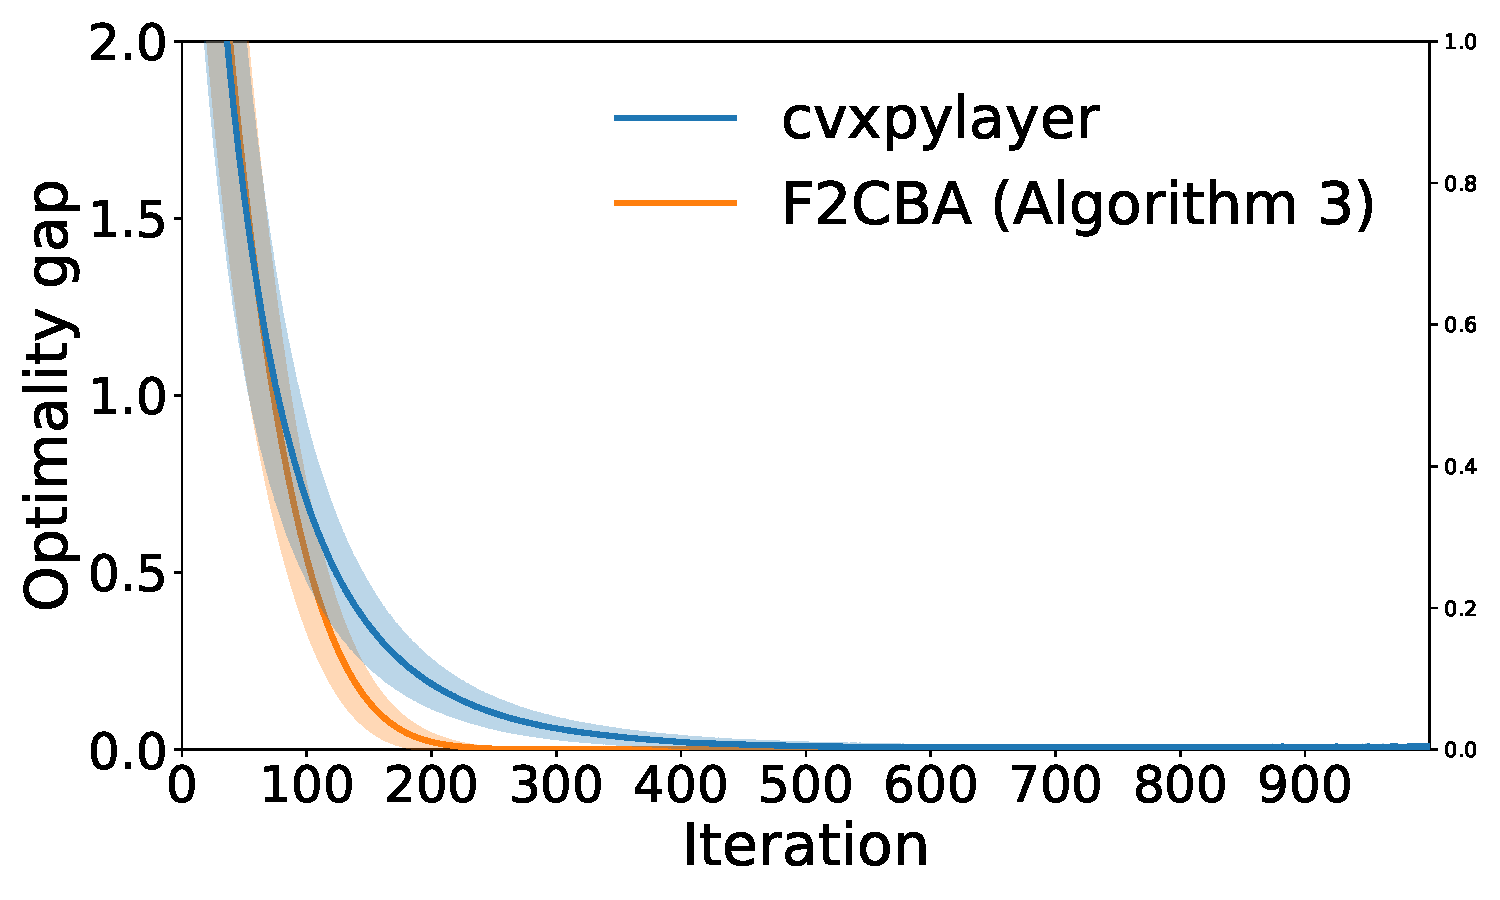
\includegraphics[width=\textwidth]{src/appendix_figures/ydim20_loss.pdf}
        \caption{Convergence and gradient error of Fully First-order Constrained Bilevel Algorithms (F2CBA). We set $d_x = 20$}
        \label{fig:convergence-comparison}
    \end{subfigure}
    \hfill
    \begin{subfigure}[b]{0.32\textwidth}
        \centering
        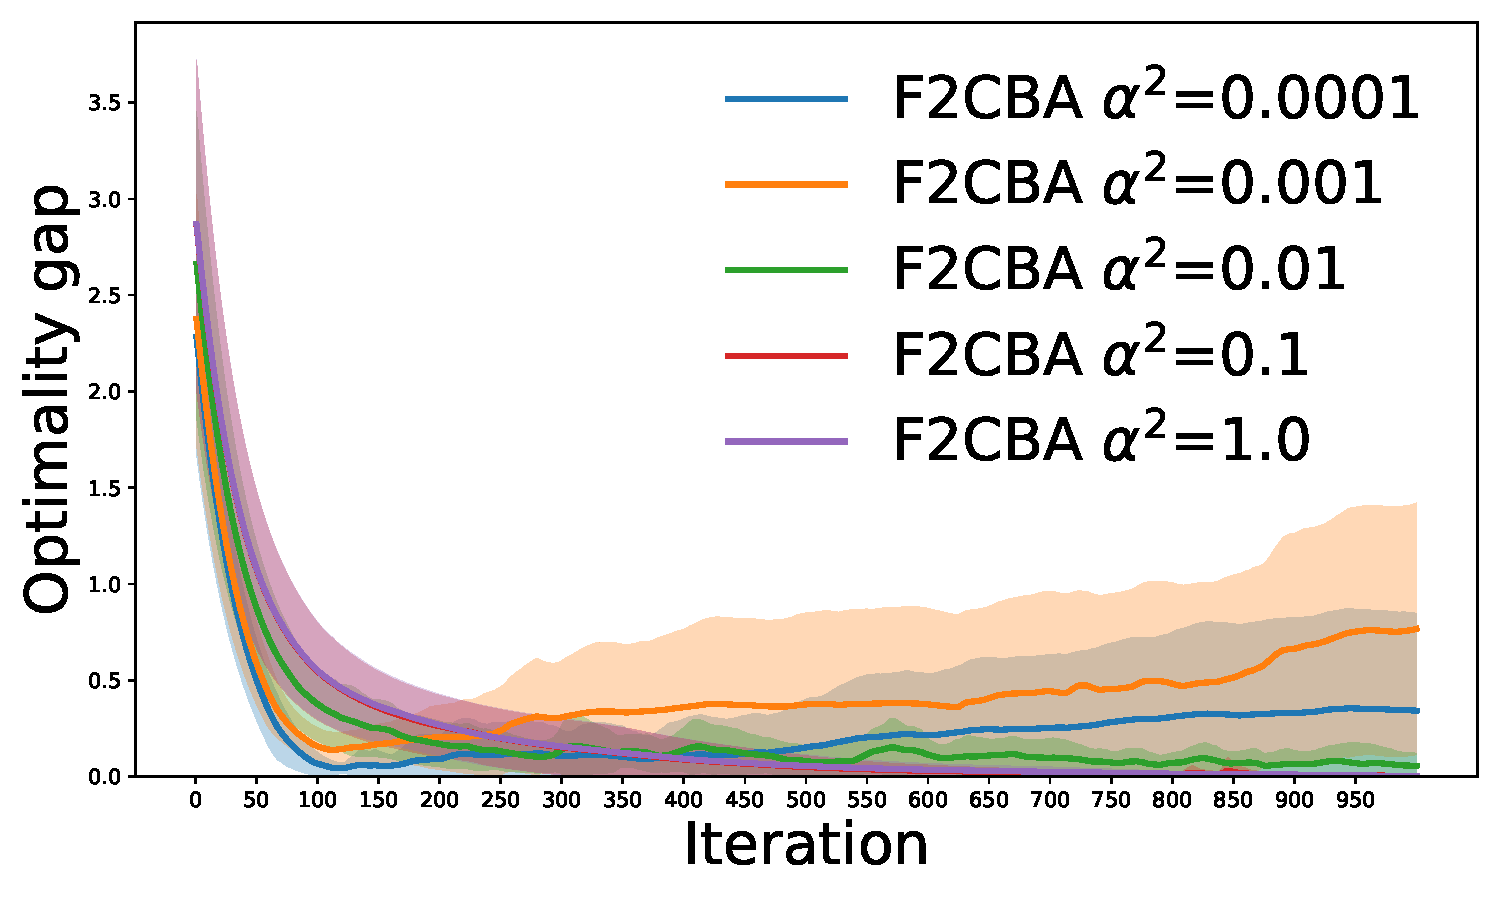
\includegraphics[width=\textwidth]{src/appendix_figures/ydim100_gradient_error.pdf}
        \caption{Convergence analysis with varying gradient inexactness $\alpha$. We set $d_x = 100$ to measure the tradeoff of accuracy and convergence.}
        \label{fig:convergence-comparison-2}
    \end{subfigure}
    \hfill
    \begin{subfigure}[b]{0.32\textwidth}
        \centering
        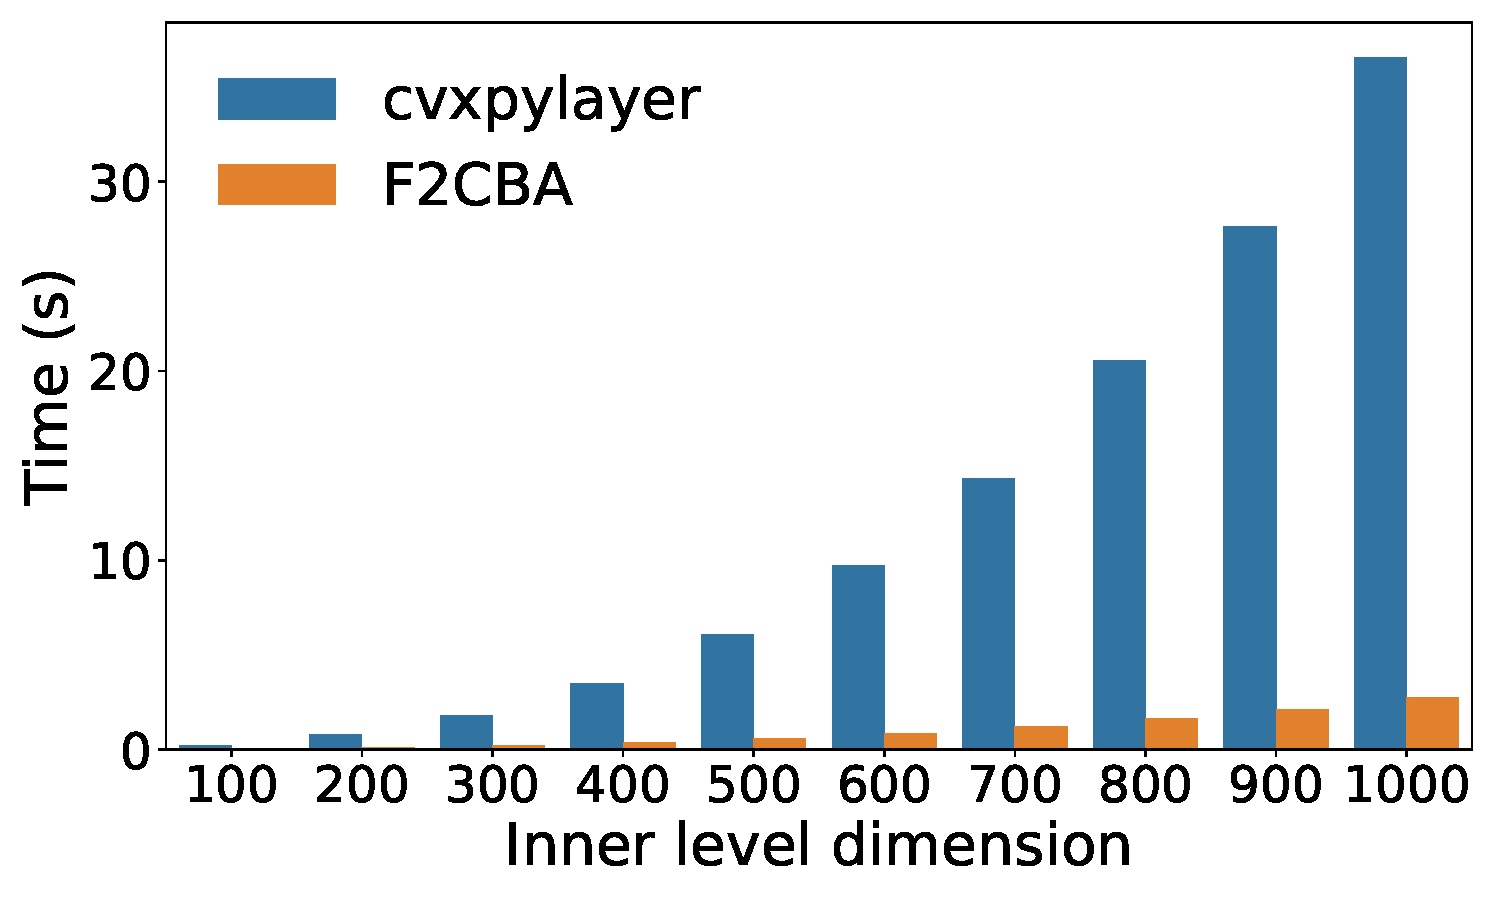
\includegraphics[width=\textwidth]{src/appendix_figures/time_results.pdf}
        \caption{Computation cost per gradient step of varying problem size $d_y$. We set $d_x = 100$ to measure large-scale computation cost.}
        \label{fig:computation-comparison}
    \end{subfigure}
    \caption{We run \cref{alg: OIGRM} using \cref{alg:inexact-gradient-oracle} on the bilevel optimization in the toy example in \cref{eqn:experiment-bilevel-optimization} with varying upper-level variable dimensions $d_x$, a fixed lower-level variable dimension $d_y = 200$, and the number of constraints $n_{\text{const}} = d_y / 5 = 40$, and accuracy $\alpha = 0.1$. \cref{fig:convergence-comparison}, \cref{fig:convergence-comparison-2}, \cref{fig:computation-comparison} vary \# of iterations, gradient exactness $\alpha$, and $d_y$, respectively, to compare the performance under different settings.}
    % Figure~\ref{fig:convergence-comparison} shows that \cref{alg: OIGRM} converges in the same rate as CvxpyLayer, while the gradient errors at each iteration are plotted in the colorful bars and are mostly below $\alpha = 0.1$ as guaranteed. Figure~\ref{fig:convergence-comparison-2} shows the convergence under different gradient inexactness $\alpha$. Figure~\ref{fig:computation-comparison} shows the computation cost of both methods under different lower level problem size $d_y$.}
    \label{fig:three graphs}
\end{figure}

We  generate instances of the following constrained bilevel optimization problem: 
\begin{align*}\numberthis\label[prob]{eqn:experiment-bilevel-optimization}
     & \mbox{minimize}_{x} ~  c^\top y^* + 0.01 \norm{x}^2 + 0.01 \norm{y^*}^2 ~\text{ subject to } ~ y^* = \argmin_{y: h(x,y) \leq 0} \frac{1}{2} y^\top Q y + x^\top P y, 
\end{align*}
% \begin{align}\label{}
%     \min\nolimits_{x} \quad & \\
%     \text{s.t.} \quad & \nonumber
% \end{align}
where $h_i(x,y) = x^\top A_i y - b_i^\top x ~\forall i \in [d_h]$ is a $d_h$-dim bilinear constraint, where the constraint bilinear matrix $A_i \in \reals^{d_x \times d_y}$, $b_i \in \reals^{d_x}$ for all $i \in [d_h]$ are randomly generated from normal distributions.
The bilinear (nonlinear) constraint of the lower-level problem is the major difference compared to the experiment in Section~\ref{sec:exp}. 
We are interested in whether our algorithms work beyond the linear constraints where our theory guarantees.

The rest of the parameters are the same as in Section~\ref{sec:exp}. The PSD matrix $Q \in \reals^{d_y \times d_y}$, $c \in \reals^{d_y}$, $P \in \reals^{d_x \times d_y}$.
We compare our \cref{alg: OIGRM} with a non-fully first-order method implemented using \texttt{cvxpyLayer}~\cite{agrawal2019differentiable}. Both algorithms use Adam~\cite{kingma2014adam} to control the learning rate in gradient descent. All the experiments are averaged over ten random seeds.



\section*{NeurIPS Paper Checklist}

% %%% BEGIN INSTRUCTIONS %%%
% The checklist is designed to encourage best practices for responsible machine learning research, addressing issues of reproducibility, transparency, research ethics, and societal impact. Do not remove the checklist: {\bf The papers not including the checklist will be desk rejected.} The checklist should follow the references and precede the (optional) supplemental material.  The checklist does NOT count towards the page
% limit. 

% Please read the checklist guidelines carefully for information on how to answer these questions. For each question in the checklist:
% \begin{itemize}
%     \item You should answer \answerYes{}, \answerNo{}, or \answerNA{}.
%     \item \answerNA{} means either that the question is Not Applicable for that particular paper or the relevant information is Not Available.
%     \item Please provide a short (1–2 sentence) justification right after your answer (even for NA). 
%    % \item {\bf The papers not including the checklist will be desk rejected.}
% \end{itemize}

% {\bf The checklist answers are an integral part of your paper submission.} They are visible to the reviewers, area chairs, senior area chairs, and ethics reviewers. You will be asked to also include it (after eventual revisions) with the final version of your paper, and its final version will be published with the paper.

% The reviewers of your paper will be asked to use the checklist as one of the factors in their evaluation. While "\answerYes{}" is generally preferable to "\answerNo{}", it is perfectly acceptable to answer "\answerNo{}" provided a proper justification is given (e.g., "error bars are not reported because it would be too computationally expensive" or "we were unable to find the license for the dataset we used"). In general, answering "\answerNo{}" or "\answerNA{}" is not grounds for rejection. While the questions are phrased in a binary way, we acknowledge that the true answer is often more nuanced, so please just use your best judgment and write a justification to elaborate. All supporting evidence can appear either in the main paper or the supplemental material, provided in appendix. If you answer \answerYes{} to a question, in the justification please point to the section(s) where related material for the question can be found.

% IMPORTANT, please:
% \begin{itemize}
%     \item {\bf Delete this instruction block, but keep the section heading ``NeurIPS paper checklist"},
%     \item  {\bf Keep the checklist subsection headings, questions/answers and guidelines below.}
%     \item {\bf Do not modify the questions and only use the provided macros for your answers}.
% \end{itemize} 
 

% %%% END INSTRUCTIONS %%%


\begin{enumerate}

\item {\bf Claims}
    \item[] Question: Do the main claims made in the abstract and introduction accurately reflect the paper's contributions and scope?
    \item[] Answer: \answerYes{} % Replace by \answerYes{}, \answerNo{}, or \answerNA{}.
    \item[] Justification: We provide algorithms and corresponding theoretical guarantees for all our claims in the abstract. We provide experiments (and relevant code) as claimed.  % \justificationTODO{}
    \item[] Guidelines:
    \begin{itemize}
        \item The answer NA means that the abstract and introduction do not include the claims made in the paper.
        \item The abstract and/or introduction should clearly state the claims made, including the contributions made in the paper and important assumptions and limitations. A No or NA answer to this question will not be perceived well by the reviewers. 
        \item The claims made should match theoretical and experimental results, and reflect how much the results can be expected to generalize to other settings. 
        \item It is fine to include aspirational goals as motivation as long as it is clear that these goals are not attained by the paper. 
    \end{itemize}

\item {\bf Limitations}
    \item[] Question: Does the paper discuss the limitations of the work performed by the authors?
    \item[] Answer: \answerYes{} % Replace by \answerYes{}, \answerNo{}, or \answerNA{}.
    \item[] Justification: This is discussed in \cref{sec:limitation}
    \item[] Guidelines:
    \begin{itemize}
        \item The answer NA means that the paper has no limitation while the answer No means that the paper has limitations, but those are not discussed in the paper. 
        \item The authors are encouraged to create a separate "Limitations" section in their paper.
        \item The paper should point out any strong assumptions and how robust the results are to violations of these assumptions (e.g., independence assumptions, noiseless settings, model well-specification, asymptotic approximations only holding locally). The authors should reflect on how these assumptions might be violated in practice and what the implications would be.
        \item The authors should reflect on the scope of the claims made, e.g., if the approach was only tested on a few datasets or with a few runs. In general, empirical results often depend on implicit assumptions, which should be articulated.
        \item The authors should reflect on the factors that influence the performance of the approach. For example, a facial recognition algorithm may perform poorly when image resolution is low or images are taken in low lighting. Or a speech-to-text system might not be used reliably to provide closed captions for online lectures because it fails to handle technical jargon.
        \item The authors should discuss the computational efficiency of the proposed algorithms and how they scale with dataset size.
        \item If applicable, the authors should discuss possible limitations of their approach to address problems of privacy and fairness.
        \item While the authors might fear that complete honesty about limitations might be used by reviewers as grounds for rejection, a worse outcome might be that reviewers discover limitations that aren't acknowledged in the paper. The authors should use their best judgment and recognize that individual actions in favor of transparency play an important role in developing norms that preserve the integrity of the community. Reviewers will be specifically instructed to not penalize honesty concerning limitations.
    \end{itemize}

\item {\bf Theory Assumptions and Proofs}
    \item[] Question: For each theoretical result, does the paper provide the full set of assumptions and a complete (and correct) proof?
    \item[] Answer: \answerYes{} % Replace by \answerYes{}, \answerNo{}, or \answerNA{}.
    \item[] Justification: The assumptions, theorem statements, and proof sketches are included in the main paper. The full proofs are included in the appendix.
    \item[] Guidelines:
    \begin{itemize}
        \item The answer NA means that the paper does not include theoretical results. 
        \item All the theorems, formulas, and proofs in the paper should be numbered and cross-referenced.
        \item All assumptions should be clearly stated or referenced in the statement of any theorems.
        \item The proofs can either appear in the main paper or the supplemental material, but if they appear in the supplemental material, the authors are encouraged to provide a short proof sketch to provide intuition. 
        \item Inversely, any informal proof provided in the core of the paper should be complemented by formal proofs provided in appendix or supplemental material.
        \item Theorems and Lemmas that the proof relies upon should be properly referenced. 
    \end{itemize}

    \item {\bf Experimental Result Reproducibility}
    \item[] Question: Does the paper fully disclose all the information needed to reproduce the main experimental results of the paper to the extent that it affects the main claims and/or conclusions of the paper (regardless of whether the code and data are provided or not)?
    \item[] Answer: \answerYes{} % Replace by \answerYes{}, \answerNo{}, or \answerNA{}.
    \item[] Justification: We provide our full code in the supplemental material, and it can be used to reproduce the experimental results.% \justificationTODO{}
    \item[] Guidelines:
    \begin{itemize}
        \item The answer NA means that the paper does not include experiments.
        \item If the paper includes experiments, a No answer to this question will not be perceived well by the reviewers: Making the paper reproducible is important, regardless of whether the code and data are provided or not.
        \item If the contribution is a dataset and/or model, the authors should describe the steps taken to make their results reproducible or verifiable. 
        \item Depending on the contribution, reproducibility can be accomplished in various ways. For example, if the contribution is a novel architecture, describing the architecture fully might suffice, or if the contribution is a specific model and empirical evaluation, it may be necessary to either make it possible for others to replicate the model with the same dataset, or provide access to the model. In general. releasing code and data is often one good way to accomplish this, but reproducibility can also be provided via detailed instructions for how to replicate the results, access to a hosted model (e.g., in the case of a large language model), releasing of a model checkpoint, or other means that are appropriate to the research performed.
        \item While NeurIPS does not require releasing code, the conference does require all submissions to provide some reasonable avenue for reproducibility, which may depend on the nature of the contribution. For example
        \begin{enumerate}
            \item If the contribution is primarily a new algorithm, the paper should make it clear how to reproduce that algorithm.
            \item If the contribution is primarily a new model architecture, the paper should describe the architecture clearly and fully.
            \item If the contribution is a new model (e.g., a large language model), then there should either be a way to access this model for reproducing the results or a way to reproduce the model (e.g., with an open-source dataset or instructions for how to construct the dataset).
            \item We recognize that reproducibility may be tricky in some cases, in which case authors are welcome to describe the particular way they provide for reproducibility. In the case of closed-source models, it may be that access to the model is limited in some way (e.g., to registered users), but it should be possible for other researchers to have some path to reproducing or verifying the results.
        \end{enumerate}
    \end{itemize}


\item {\bf Open access to data and code}
    \item[] Question: Does the paper provide open access to the data and code, with sufficient instructions to faithfully reproduce the main experimental results, as described in supplemental material?
    \item[] Answer: \answerYes{} % Replace by \answerYes{}, \answerNo{}, or \answerNA{}.
    \item[] Justification: The code is included in the supplemental material and can be used to reproduce the experiments.
    \item[] Guidelines:
    \begin{itemize}
        \item The answer NA means that paper does not include experiments requiring code.
        \item Please see the NeurIPS code and data submission guidelines (\url{https://nips.cc/public/guides/CodeSubmissionPolicy}) for more details.
        \item While we encourage the release of code and data, we understand that this might not be possible, so “No” is an acceptable answer. Papers cannot be rejected simply for not including code, unless this is central to the contribution (e.g., for a new open-source benchmark).
        \item The instructions should contain the exact command and environment needed to run to reproduce the results. See the NeurIPS code and data submission guidelines (\url{https://nips.cc/public/guides/CodeSubmissionPolicy}) for more details.
        \item The authors should provide instructions on data access and preparation, including how to access the raw data, preprocessed data, intermediate data, and generated data, etc.
        \item The authors should provide scripts to reproduce all experimental results for the new proposed method and baselines. If only a subset of experiments are reproducible, they should state which ones are omitted from the script and why.
        \item At submission time, to preserve anonymity, the authors should release anonymized versions (if applicable).
        \item Providing as much information as possible in supplemental material (appended to the paper) is recommended, but including URLs to data and code is permitted.
    \end{itemize}


\item {\bf Experimental Setting/Details}
    \item[] Question: Does the paper specify all the training and test details (e.g., data splits, hyperparameters, how they were chosen, type of optimizer, etc.) necessary to understand the results?
    \item[] Answer: \answerYes{}%\answerTODO{} % Replace by \answerYes{}, \answerNo{}, or \answerNA{}.
    \item[] Justification: We provide this information in \cref{{appendix:experiment-setup}}.%\justificationTODO{}
    \item[] Guidelines:
    \begin{itemize}
        \item The answer NA means that the paper does not include experiments.
        \item The experimental setting should be presented in the core of the paper to a level of detail that is necessary to appreciate the results and make sense of them.
        \item The full details can be provided either with the code, in appendix, or as supplemental material.
    \end{itemize}

\item {\bf Experiment Statistical Significance}
    \item[] Question: Does the paper report error bars suitably and correctly defined or other appropriate information about the statistical significance of the experiments?
    \item[] Answer: \answerYes{}% \answerTODO{} % Replace by \answerYes{}, \answerNo{}, or \answerNA{}.
    \item[] Justification: We provide this in \cref{sec:exp} %\justificationTODO{}
    \item[] Guidelines:
    \begin{itemize}
        \item The answer NA means that the paper does not include experiments.
        \item The authors should answer "Yes" if the results are accompanied by error bars, confidence intervals, or statistical significance tests, at least for the experiments that support the main claims of the paper.
        \item The factors of variability that the error bars are capturing should be clearly stated (for example, train/test split, initialization, random drawing of some parameter, or overall run with given experimental conditions).
        \item The method for calculating the error bars should be explained (closed form formula, call to a library function, bootstrap, etc.)
        \item The assumptions made should be given (e.g., Normally distributed errors).
        \item It should be clear whether the error bar is the standard deviation or the standard error of the mean.
        \item It is OK to report 1-sigma error bars, but one should state it. The authors should preferably report a 2-sigma error bar than state that they have a 96\% CI, if the hypothesis of Normality of errors is not verified.
        \item For asymmetric distributions, the authors should be careful not to show in tables or figures symmetric error bars that would yield results that are out of range (e.g. negative error rates).
        \item If error bars are reported in tables or plots, The authors should explain in the text how they were calculated and reference the corresponding figures or tables in the text.
    \end{itemize}

\item {\bf Experiments Compute Resources}
    \item[] Question: For each experiment, does the paper provide sufficient information on the computer resources (type of compute workers, memory, time of execution) needed to reproduce the experiments?
    \item[] Answer: \answerYes{}% \answerTODO{} % Replace by \answerYes{}, \answerNo{}, or \answerNA{}.
    \item[] Justification: We provide this information in \cref{{appendix:experiment-setup}}. %\justificationTODO{}
    \item[] Guidelines:
    \begin{itemize}
        \item The answer NA means that the paper does not include experiments.
        \item The paper should indicate the type of compute workers CPU or GPU, internal cluster, or cloud provider, including relevant memory and storage.
        \item The paper should provide the amount of compute required for each of the individual experimental runs as well as estimate the total compute. 
        \item The paper should disclose whether the full research project required more compute than the experiments reported in the paper (e.g., preliminary or failed experiments that didn't make it into the paper). 
    \end{itemize}
    
\item {\bf Code Of Ethics}
    \item[] Question: Does the research conducted in the paper conform, in every respect, with the NeurIPS Code of Ethics \url{https://neurips.cc/public/EthicsGuidelines}?
    \item[] Answer: \answerYes{}% \answerTODO{} % Replace by \answerYes{}, \answerNo{}, or \answerNA{}.
    \item[] Justification: Yes, the research conducted in the paper conforms, in every respect, with the NeurIPS Code of Ethics. %\justificationTODO{}
    \item[] Guidelines:
    \begin{itemize}
        \item The answer NA means that the authors have not reviewed the NeurIPS Code of Ethics.
        \item If the authors answer No, they should explain the special circumstances that require a deviation from the Code of Ethics.
        \item The authors should make sure to preserve anonymity (e.g., if there is a special consideration due to laws or regulations in their jurisdiction).
    \end{itemize}


\item {\bf Broader Impacts}
    \item[] Question: Does the paper discuss both potential positive societal impacts and negative societal impacts of the work performed?
    \item[] Answer: \answerNA{}% \answerTODO{} % Replace by \answerYes{}, \answerNo{}, or \answerNA{}.
    \item[] Justification: There is no societal impact of this work.% \justificationTODO{}
    \item[] Guidelines:
    \begin{itemize}
        \item The answer NA means that there is no societal impact of the work performed.
        \item If the authors answer NA or No, they should explain why their work has no societal impact or why the paper does not address societal impact.
        \item Examples of negative societal impacts include potential malicious or unintended uses (e.g., disinformation, generating fake profiles, surveillance), fairness considerations (e.g., deployment of technologies that could make decisions that unfairly impact specific groups), privacy considerations, and security considerations.
        \item The conference expects that many papers will be foundational research and not tied to particular applications, let alone deployments. However, if there is a direct path to any negative applications, the authors should point it out. For example, it is legitimate to point out that an improvement in the quality of generative models could be used to generate deepfakes for disinformation. On the other hand, it is not needed to point out that a generic algorithm for optimizing neural networks could enable people to train models that generate Deepfakes faster.
        \item The authors should consider possible harms that could arise when the technology is being used as intended and functioning correctly, harms that could arise when the technology is being used as intended but gives incorrect results, and harms following from (intentional or unintentional) misuse of the technology.
        \item If there are negative societal impacts, the authors could also discuss possible mitigation strategies (e.g., gated release of models, providing defenses in addition to attacks, mechanisms for monitoring misuse, mechanisms to monitor how a system learns from feedback over time, improving the efficiency and accessibility of ML).
    \end{itemize}
    
\item {\bf Safeguards}
    \item[] Question: Does the paper describe safeguards that have been put in place for responsible release of data or models that have a high risk for misuse (e.g., pretrained language models, image generators, or scraped datasets)?
    \item[] Answer: \answerNA{}% \answerTODO{} % Replace by \answerYes{}, \answerNo{}, or \answerNA{}.
    \item[] Justification: The paper poses no such risks.% \justificationTODO{}
    \item[] Guidelines:
    \begin{itemize}
        \item The answer NA means that the paper poses no such risks.
        \item Released models that have a high risk for misuse or dual-use should be released with necessary safeguards to allow for controlled use of the model, for example by requiring that users adhere to usage guidelines or restrictions to access the model or implementing safety filters. 
        \item Datasets that have been scraped from the Internet could pose safety risks. The authors should describe how they avoided releasing unsafe images.
        \item We recognize that providing effective safeguards is challenging, and many papers do not require this, but we encourage authors to take this into account and make a best faith effort.
    \end{itemize}

\item {\bf Licenses for existing assets}
    \item[] Question: Are the creators or original owners of assets (e.g., code, data, models), used in the paper, properly credited and are the license and terms of use explicitly mentioned and properly respected?
    \item[] Answer: \answerNA{}% \answerTODO{} % Replace by \answerYes{}, \answerNo{}, or \answerNA{}.
    \item[] Justification: The paper does not use existing assets.% \justificationTODO{}
    \item[] Guidelines:
    \begin{itemize}
        \item The answer NA means that the paper does not use existing assets.
        \item The authors should cite the original paper that produced the code package or dataset.
        \item The authors should state which version of the asset is used and, if possible, include a URL.
        \item The name of the license (e.g., CC-BY 4.0) should be included for each asset.
        \item For scraped data from a particular source (e.g., website), the copyright and terms of service of that source should be provided.
        \item If assets are released, the license, copyright information, and terms of use in the package should be provided. For popular datasets, \url{paperswithcode.com/datasets} has curated licenses for some datasets. Their licensing guide can help determine the license of a dataset.
        \item For existing datasets that are re-packaged, both the original license and the license of the derived asset (if it has changed) should be provided.
        \item If this information is not available online, the authors are encouraged to reach out to the asset's creators.
    \end{itemize}

\item {\bf New Assets}
    \item[] Question: Are new assets introduced in the paper well documented and is the documentation provided alongside the assets?
    \item[] Answer: \answerNA{} %\answerTODO{} % Replace by \answerYes{}, \answerNo{}, or \answerNA{}.
    \item[] Justification: The paper does not release new assets.% \justificationTODO{}
    \item[] Guidelines:
    \begin{itemize}
        \item The answer NA means that the paper does not release new assets.
        \item Researchers should communicate the details of the dataset/code/model as part of their submissions via structured templates. This includes details about training, license, limitations, etc. 
        \item The paper should discuss whether and how consent was obtained from people whose asset is used.
        \item At submission time, remember to anonymize your assets (if applicable). You can either create an anonymized URL or include an anonymized zip file.
    \end{itemize}

\item {\bf Crowdsourcing and Research with Human Subjects}
    \item[] Question: For crowdsourcing experiments and research with human subjects, does the paper include the full text of instructions given to participants and screenshots, if applicable, as well as details about compensation (if any)? 
    \item[] Answer: \answerNA{}% \answerTODO{} % Replace by \answerYes{}, \answerNo{}, or \answerNA{}.
    \item[] Justification: No crowdsourcing or research with human subjects is involved. %\justificationTODO{}
    \item[] Guidelines:
    \begin{itemize}
        \item The answer NA means that the paper does not involve crowdsourcing nor research with human subjects.
        \item Including this information in the supplemental material is fine, but if the main contribution of the paper involves human subjects, then as much detail as possible should be included in the main paper. 
        \item According to the NeurIPS Code of Ethics, workers involved in data collection, curation, or other labor should be paid at least the minimum wage in the country of the data collector. 
    \end{itemize}

\item {\bf Institutional Review Board (IRB) Approvals or Equivalent for Research with Human Subjects}
    \item[] Question: Does the paper describe potential risks incurred by study participants, whether such risks were disclosed to the subjects, and whether Institutional Review Board (IRB) approvals (or an equivalent approval/review based on the requirements of your country or institution) were obtained?
    \item[] Answer: \answerNA{} %\answerTODO{} % Replace by \answerYes{}, \answerNo{}, or \answerNA{}.
    \item[] Justification: The paper does not involve crowdsourcing nor research with human subjects.% \justificationTODO{}
    \item[] Guidelines:
    \begin{itemize}
        \item The answer NA means that the paper does not involve crowdsourcing nor research with human subjects.
        \item Depending on the country in which research is conducted, IRB approval (or equivalent) may be required for any human subjects research. If you obtained IRB approval, you should clearly state this in the paper. 
        \item We recognize that the procedures for this may vary significantly between institutions and locations, and we expect authors to adhere to the NeurIPS Code of Ethics and the guidelines for their institution. 
        \item For initial submissions, do not include any information that would break anonymity (if applicable), such as the institution conducting the review.
    \end{itemize}

\end{enumerate}